\documentclass[a4paper,12pt]{extarticle}

\pdfmapfile{pscyr.map}
\renewcommand{\rmdefault}{ftm}


\usepackage[titletoc]{appendix}
\usepackage{indentfirst}
\usepackage[T2A]{fontenc}
\usepackage[utf8]{inputenc}
\usepackage[russian]{babel}
\usepackage{graphicx}
\usepackage{titlesec}
\usepackage{enumerate}
\usepackage{enumitem}
\usepackage{cleveref}
\usepackage[tableposition=top]{caption}
\usepackage{subcaption}
\usepackage{chngcntr}
\usepackage{float}
\usepackage{textcase} 
\usepackage{tocloft}
\usepackage{listings}
\usepackage{lastpage}
\usepackage{soulutf8}
\usepackage[figure,table,section]{totalcount}
\usepackage[section]{placeins}
\usepackage{pdfpages}
\usepackage{cleveref}
\usepackage{algorithm}
\usepackage{tabularx}
\usepackage{multirow}
\usepackage{makecell}
\usepackage{tikz}
\usepackage{pgfplots}
\usepackage{courier}
\usepackage{microtype}
\usepackage[scaled]{beramono}
\usepackage{ifthen}
\usepackage{varwidth}
\usetikzlibrary{shapes,arrows,matrix}
\usepackage{geometry} % Меняем поля страницы
\geometry{left=2.5cm}% левое поле
\geometry{right=1.5cm}% правое поле
\geometry{top=2cm}% верхнее поле
\geometry{bottom=2cm}% нижнее поле

\newcommand\myappendix[1]{

\refstepcounter{section}

\section*{Приложение~\thesection{}~#1}

\addcontentsline{toc}{section}{~\thesection{}~#1}}

% Для списков
% \renewcommand{\labelenumi}{-}
% \renewcommand{\labelenumii}{\arabic{enumii})}
% \renewcommand{\labelenumiii}{\arabic{enumii}.\arabic{enumiii})}

\setlength\parindent{1.27cm}

\makeatletter
\AddEnumerateCounter{\asbuk}{\russian@alph}{щ}
\makeatother

\newlength\myfntht
\newcommand{\myfontsize}[2][1.2]{\setlength\myfntht{#2}%
	\fontsize{\myfntht}{#1\myfntht}\selectfont}

% Отступы для списков.
%\setenumerate[1]{label=\asbuk*), ref=\asbuk*, fullwidth, itemindent=\parindent, leftmargin=0\parindent, topsep=0pt}

\setenumerate[1]{label=-, fullwidth, itemindent=\parindent, leftmargin=0\parindent, topsep=0pt, itemsep=-5pt}

\setenumerate[2]{label=\arabic{enumii}), fullwidth, itemindent=1\parindent, leftmargin=1\parindent}

\setenumerate[3]{label=\arabic{enumii}.\arabic{enumiii}), fullwidth, itemindent=1\parindent, leftmargin=1\parindent}

% Межстрочный интервал
\renewcommand{\baselinestretch}{1.25}

\sloppy

%Частота переносов
\hyphenpenalty=2000

%Висячие строки
\clubpenalty=10000
\widowpenalty=10000

% Нумерация страниц сверху
\pagestyle{myheadings}

%Точки в содержании
\renewcommand{\cftsecleader}{\cftdotfill{\cftdotsep}}

\linespread{1.3}
\frenchspacing

\newlength{\normalparindent}
\AtBeginDocument{\setlength{\normalparindent}{\parindent}}

\titlespacing*{\chapter}
  {0pt}{0ex}{1\baselineskip}
\titlespacing*{\section}
  {0pt}{0ex}{1\baselineskip}
\titlespacing*{\subsection}
  {0pt}{2\baselineskip}{2\baselineskip}
  \titlespacing*{\subsubsection}
  {0pt}{2\baselineskip}{2\baselineskip}

% 
\titleformat{\chapter}[block]
  {\centering}
  {\hspace*{\normalparindent}\thechapter}
  {1ex}
  {}

\titleformat{\section}[block]
  {\centering}
  {\hspace*{\normalparindent}\thesection}
  {1ex}
  {}

\titleformat{\subsection}[block]
  {}
  {\hspace*{\normalparindent}\thesubsection}
  {1ex}
  {}
  
\titleformat{\subsubsection}[block]
  {}
  {\hspace*{\normalparindent}\thesubsubsection}
  {1ex}
  {}
 

% 
%\allsectionsfont{\normalsize}

 
\DeclareCaptionLabelFormat{gostfigure}{Рисунок #2}
\DeclareCaptionLabelFormat{gosttable}{Таблица #2}
\DeclareCaptionLabelSeparator{gost}{~---~}
\captionsetup{labelsep=gost}
\captionsetup[figure]{labelformat=gostfigure}
\captionsetup[table]{labelformat=gosttable}
\renewcommand{\thesubfigure}{\asbuk{subfigure}}

\newcommand{\crefrangeconjunction}{-}
\crefname{table}{см. рис.}{см. рис.}

%For counting
\counterwithin{figure}{section}
\counterwithin{table}{section}

\graphicspath{ {img/} }

\newcommand{\addimg}[4]{
\begin{figure}[!htb]
    \centering
    \captionsetup{justification=centering}
    \includegraphics[scale=#2]{#1}
    \caption{#3}
    \label{fig:#4}
\end{figure}
}

\newcommand{\addtable}[3]{
	\begin{table}[!htb]
		\centering
		\captionsetup{justification=centering}
		\caption{#1}
		#3	
		\label{table:#2}
	\end{table}
}

\crefformat{figure}{см. рис. #1}
\crefformat{table}{см. табл. #1}

\newcommand\Small{\fontsize{9}{9.2}\selectfont}
\newcommand*\LSTfont{\Small\ttfamily\SetTracking{encoding=*}{-60}\lsstyle}

\lstset { 
	language=C++,
	basicstyle=\LSTfont,
	tabsize=2
}

%%%%% Tikz settings for grids

\tikzset{>=latex}

\pgfkeys{
	mygrid/.is family,
	mygrid,
	width/.initial=2,
	height/.initial=2,
	step/.initial=1,
	color/.initial=black,
}
\newcommand\mygridset[1]{\pgfkeys{mygrid,#1}}
\newcommand\mygrid[1][]{
	\mygridset{#1,
		width/.get=\gridwidth,
		height/.get=\gridheight,
		step/.get=\gridstep,
		color/.get=\gridcolor
	}
	
	\draw [step=\gridstep, thick,\gridcolor]
	(0,0) grid (\gridwidth,\gridheight);
}

\pgfkeys{
	mybox/.is family,
	mybox,
	x/.initial=0.5,
	y/.initial=0.5,
	color/.initial=blue,
}

\newcommand\myboxset[1]{\pgfkeys{mybox,#1}}
\newcommand\mybox[1][]{
	\myboxset{#1,
		x/.get=\boxx,
		y/.get=\boxy,
		color/.get=\boxcolor
	}
	\node[rectangle, minimum size=1cm, fill=\boxcolor, draw=none] at (\boxx + 0.5, \boxy + 0.5){};
}

\pgfkeys{
	myarrow/.is family,
	myarrow,
	startx/.initial=0.5,
	starty/.initial=0.5,
	endx/.initial=1.5,
	endy/.initial=1.5,
	color/.initial=red,
}

\newcommand\myarrowset[1]{\pgfkeys{myarrow,#1}}
\newcommand\myarrow[1][]{
	\myarrowset{#1,
		startx/.get=\arrowstartx,
		starty/.get=\arrowstarty,
		endx/.get=\arrowendx,
		endy/.get=\arrowendy,
		color/.get=\arrowcolor
	}
		
	\draw[line width=0.1cm,->,shorten <=0.2cm, \arrowcolor] (\arrowstartx + 0.5, \arrowstarty + 0.5) -- (\arrowendx + 0.5, \arrowendy + 0.5);	
}

\definecolor{grey}{RGB}{200,200,200}
\definecolor{darkgrey}{RGB}{110,110,110}

\newcommand{\addtikz}[4]{
	\begin{figure}[!htb]
		\centering
		\captionsetup{justification=centering}
		
		\begin{tikzpicture}[scale=#3, every node/.style={scale=#3}]
		#4
		\end{tikzpicture}
		
		\caption{#1}
		\label{fig:#2}
	\end{figure}
}

%%%%% End tikz settings 

\makeatletter
\renewenvironment{thebibliography}[1]
{\list{\@arabic\c@enumiv.}%
    {\settowidth\labelwidth{\@biblabel{#1}}%
    	\topsep=0pt
        \leftmargin=0pt
        \itemindent=1.5\parindent	% Костыль
        \itemsep=-5pt	% Костыль
        \@openbib@code
        \usecounter{enumiv}%
        \let\p@enumiv\@empty
        \renewcommand\theenumiv{\@arabic\c@enumiv}}%
    \sloppy
    \clubpenalty4000
    \@clubpenalty \clubpenalty
    \widowpenalty4000%
    \sfcode`\.\@m}
{\def\@noitemerr
    {\@latex@warning{Empty `thebibliography' environment}}%
    \endlist}
\makeatother

\newcounter{mycite}
\newtoks\citetoks
\makeatletter
\DeclareRobustCommand\unscite[1]{%
	\@ifundefined{uns@cite#1}
	{\refstepcounter{mycite}\label{citelabel@#1}%
		\expandafter\xdef\csname uns@cite#1\endcsname{\arabic{mycite}}%
		\toks\z@=\expandafter{\the\citetoks}%
		\toks\tw@=\expandafter\expandafter\expandafter{%
			\csname uns@bibitem#1\endcsname}%
		\edef\@tempcite{\the\toks\z@\the\toks\tw@}%
		\global\citetoks=\expandafter{\@tempcite}%
	}{}[\@nameuse{uns@cite#1}]}
\newcommand{\orderedbibitem}[2]{%
	\@namedef{uns@bibitem#1}{\bibitem{#1}#2}}
\makeatother

\renewcommand{\cite}{\unscite}

\orderedbibitem{Dijkstra}{Алгоритмы: построение и анализ. Второе издание [Текст] / Х. Т. Кормен, Ч. И. Лейзерсон , Р. Л. Ривест, К. Штайн - М.: ``Вильямс'', 2006. - 1296 с. - ISBN 0-07-013151-1.}

\orderedbibitem{A_STAR}{Russell S. Artificial Intelligence: A Modern Approach [Текст] / S. Russell, Norvig P. - Prentice Hall, 2009. - 1152 с. - ISBN 978-0-13-604259-4.}

\orderedbibitem{HPA}{Botea A. Near Optimal Hierarchical Path-Finding [Текст] / A. Botea, M. Muller, J. Schaeffer // Журн. Journal of Game Development. - 2011. №1.}

\orderedbibitem{IMPROVING_JPS}{
	Harabor D. D.  Improving Jump Point Search. Pathfinding Algorithm [Текст] / D. D. Harabor, A. Grastien // тез.докл.науч.-практ. конф. ICAPS. -- 2015. }

\orderedbibitem{HEURISTICS}{
   	Информационный портал stanford.edu - Heuristics From Amit’s Thoughts on Pathfinding [Электронный ресурс]: -- Режим доступа: https://theory.stanford.edu/~amitp/GameProgramming/Heuristics.html - Загл. с экрана.}

\orderedbibitem{GOAL_BOUNDING}{
   	Репозиторий кода GitHub - Steve Rabin JPS+ and Goal Bounding [Электронный ресурс]: -- Режим доступа: https://www.github.com/SteveRabin/JPSPlusWithGoalBounding/ - Загл. с экрана.}

\orderedbibitem{UML_USER_GUIDE_2ND}{
   	Booch G. Unified Modeling Language User Guide, The, 2nd Edition [Текст]
   	/ G. Booch, J. Rumbaugh, I. Jacobson - Addison-Wesley, 2005. - 496 с. - ISBN 0-321-26797-4.}
   
\orderedbibitem{THREAD_POOL}{
   	Mattson T. Patterns for Parallel Programming [Текст]
   	/ T. Mattson, S. Beverly, B. Massingill - Addison-Wesley, 2005. - 355 с. - ISBN 0-321-22811-1.}

\begin{document}

%\thispagestyle{empty}

{
\centering{
	\textbf{
		\myfontsize{14pt}{МІНІСТЕРСТВО ОСВІТИ І НАУКИ УКРАЇНИ	}}


	\textbf{
		\myfontsize{13pt}{ХАРКІВСЬКИЙ НАЦІОНАЛЬНИЙ УНІВЕРСИТЕТ РАДІОЕЛЕКТРОНІКИ }}
	
	\vspace{1\baselineskip}
	
	\myfontsize{14pt}{
	
		Факультет комп’ютерних наук
		
		\vspace{2\baselineskip}
		
		Кафедра Програмної інженерії
		
		\vspace{2\baselineskip}
		
		\textbf{ВИПУСКНА КВАЛІФІКАЦІЙНА РОБОТА БАКАЛАВРА}
		
		\vspace{4\baselineskip}}
	
\myfontsize{16pt}{ Програма пошуку найкоротшого шляху для iгрових додаткiв }


\myfontsize{8pt}{(Тема  роботи)}

\vspace{1\baselineskip}

\myfontsize{14pt}{\quad\quad Студент гр.  ПІ-12-1 \hfill Піляєв Д.В. \quad \quad}

\vspace{-0.5\baselineskip}

\flushleft{
\myfontsize{10pt}{\hspace{10em} позначка групи \hspace{21em}  Прізвище, ініціали }	}

\vspace{1\baselineskip}

\myfontsize{14pt}{\quad\quad Керівник роботи, проф. \hfill Качко О.Г. \hspace{1em} \quad}

\vspace{-0.5\baselineskip}

\flushleft{
	\myfontsize{10pt}{\hspace{14em} звання \hspace{21em}  Прізвище, ініціали }	}


\vspace{4\baselineskip}

\flushleft{\myfontsize{14pt}{\quad\quad\textbf{Допускається до захисту}}}

\flushleft{
	\myfontsize{14pt}{\quad\quad Зав. кафедри, проф. \quad\quad \quad  \rule[-0.7ex]{8em}{.3pt} \hfil \underline{\hspace{2em} З. В.Дудар \hspace{2em}} }
}

\vfill
\centering{
2016 р.}

}
}

\newpage
%
%\thispagestyle{empty}

{
	
\myfontsize{12pt}{
\centering{	\textbf{
	ХАРКІВСЬКИЙ НАЦІОНАЛЬНИЙ УНІВЕРСИТЕТ РАДІОЕЛЕКТРОНІКИ }}	
	
\vspace{1\baselineskip}

\underline{Факультет комп’ютерних наук} \hfill \underline{Кафедра програмної інженерії} \quad
	
\flushleft	
\textbf{Напрям} \underline{6.050103 «Програмна інженерія»}

\vspace{1\baselineskip}

\hfill\begin{minipage}{0.4\linewidth}
	\centering
	
	ЗАТВЕРДЖУЮ:
	
	\ul{\mbox{\hspace{9em}}}
	
	"\ul{\mbox{\hspace{2em}}}" \ul{\mbox{\hspace{4em}}}20\ul{\mbox{\hspace{1.5em}}}р
	
	Зав. кафедри проф. З.В.Дудар
\end{minipage}

\vspace{2\baselineskip}

\centering{ 	\textbf{ЗАВДАННЯ}
		
	\textbf{НА ВИПУСКНУ КВАЛІФІКАЦІЙНУ РОБОТУ БАКАЛАВРА СТУДЕНТОВІ }
}

\centering{\underline{Піляєв Данило Вікторович}}
%\underline{\hspace{\linewidth}}

\centering{\myfontsize{8pt}{Прізвище, ім’я, по батькові} }

\vspace{1\baselineskip}

\begin{enumerate}
	[
	labelindent=*,
	style=multiline,
	leftmargin=*,
	label=\arabic*.
	]
	
	\item Тема роботи «Програма пошуку найкоротшого шляху для ігрових додатків» затверджена наказом університету № \underline{\quad NNN \quad} від «\ul{15}» \ul{травня} 2016 р.
	
	\item Термін здачі студентом закінченої роботи «\ul{15}» \ul{червня} 2016 р.
	
	\item Вихідні дані до роботи: \ul{розробити програму пошуку найкоротшого шляху для ігрових додатків, використовуючи мову C++}
	
	\item Зміст пояснювальної записки:
	
	\item Перелік графічного матеріалу (назви слайдів презентації)
\end{enumerate}

}
}

\newpage
\thispagestyle{empty}

\begin{enumerate}
	[
	labelindent=*,
	style=multiline,
	leftmargin=*,
	label=\arabic*.
	]
	\setcounter{enumi}{5}
	
	\item Консультанти з (роботи) із зазначенням розділів проекту, що їх стосуються
	
	\begin{table}[!h]
	\begin{tabularx}{\textwidth}{XXXXl}
		\cline{1-4}
		\multicolumn{1}{|l|}{\multirow{2}{*}{Розділ}} & \multicolumn{1}{l|}{\multirow{2}{*}{Консультант}} & \multicolumn{2}{l|}{Підпис, дата}                                           &  \\ \cline{3-4}
		\multicolumn{1}{|l|}{}                        & \multicolumn{1}{l|}{}                             & \multicolumn{1}{l|}{Завдання видав} & \multicolumn{1}{l|}{Завдання прийняв} &  \\ \cline{1-4}
		\multicolumn{1}{|l|}{Спецчастина}             & \multicolumn{1}{l|}{}                             & \multicolumn{1}{l|}{Качко О.Г.}     & \multicolumn{1}{l|}{}                 &  \\ \cline{1-4}
		&                                                   &                                     &                                       & 
	\end{tabularx}
	\end{table}
	
	\item Календарний план
	
	\begin{table}[!h]
	\begin{tabularx}{0.975\textwidth}{|l|p{6.5cm}|p{4cm}|X|}
		\hline
		№ & Назва етапів бакалаврської роботи & Термін виконання & \myfontsize{10pt}{\thead{Позначка керівника\\ про реальний строк\\ виконання}} \\ \hline
		1 & & «20» квітня 2016р \newline \myfontsize{8pt}{День початку практики}   &        \\ \hline
		2 & & «20» квітня 2016р  &        \\ \hline
		3 & & «20» квітня 2016р  &        \\ \hline
		4 & & «20» квітня 2016р  &        \\ \hline
		5 & & «20» квітня 2016р  &        \\ \hline
		6 & & «20» квітня 2016р  &        \\ \hline
		7 & Підготовка пояснювальної записки. & «20» квітня 2016р  &        \\ \hline
		8 & Спецчастина & «20» квітня 2016р &    \\ \hline
		9 & Підготовка презентації та доповіді  & «20» квітня 2016р & \\ \hline
		10 & Рецензування  & «20» квітня 2016р \newline \myfontsize{8pt}{за два тижня до початку захистів} & \\ \hline
		11 & Попередній захист   & «20» квітня 2016р \newline \myfontsize{8pt}{за тиждень до початку захистів} & \\ \hline
		12 & Занесення диплома в електронний архів   & «20» квітня 2016р \newline \myfontsize{8pt}{за 5 днів до початку роботи ДЕК} & \\ \hline
		13 & Допуск до захисту у зав. кафедри & «20» квітня 2016р \newline \myfontsize{8pt}{за 3 дні до початку роботи ДЕК} & \\ \hline
	\end{tabularx}
	\end{table}
\end{enumerate}

Дата видачі завдання «\underline{20}» квітня 2016 р.

Керівник \ul{\mbox{\hspace{5em}}} \hspace{7em} \ul{\mbox{\hspace{6em}}} \hspace{1em} \ul{\mbox{\hspace{8em}}}

\hspace{4em} {\myfontsize{8pt}{посада, звання}} \hspace{17em} {\myfontsize{8pt}{Прізвище, ініціал}}

\vspace{1\baselineskip}

Завдання прийняв до виконання \hspace{2.5em} \ul{\mbox{\hspace{6em}}} \hspace{1em} \ul{\mbox{\hspace{8em}}}

\hspace{26em} {\myfontsize{8pt}{Прізвище, ініціал}}

\newpage


\includepdf[pages=1]{title_new.pdf}

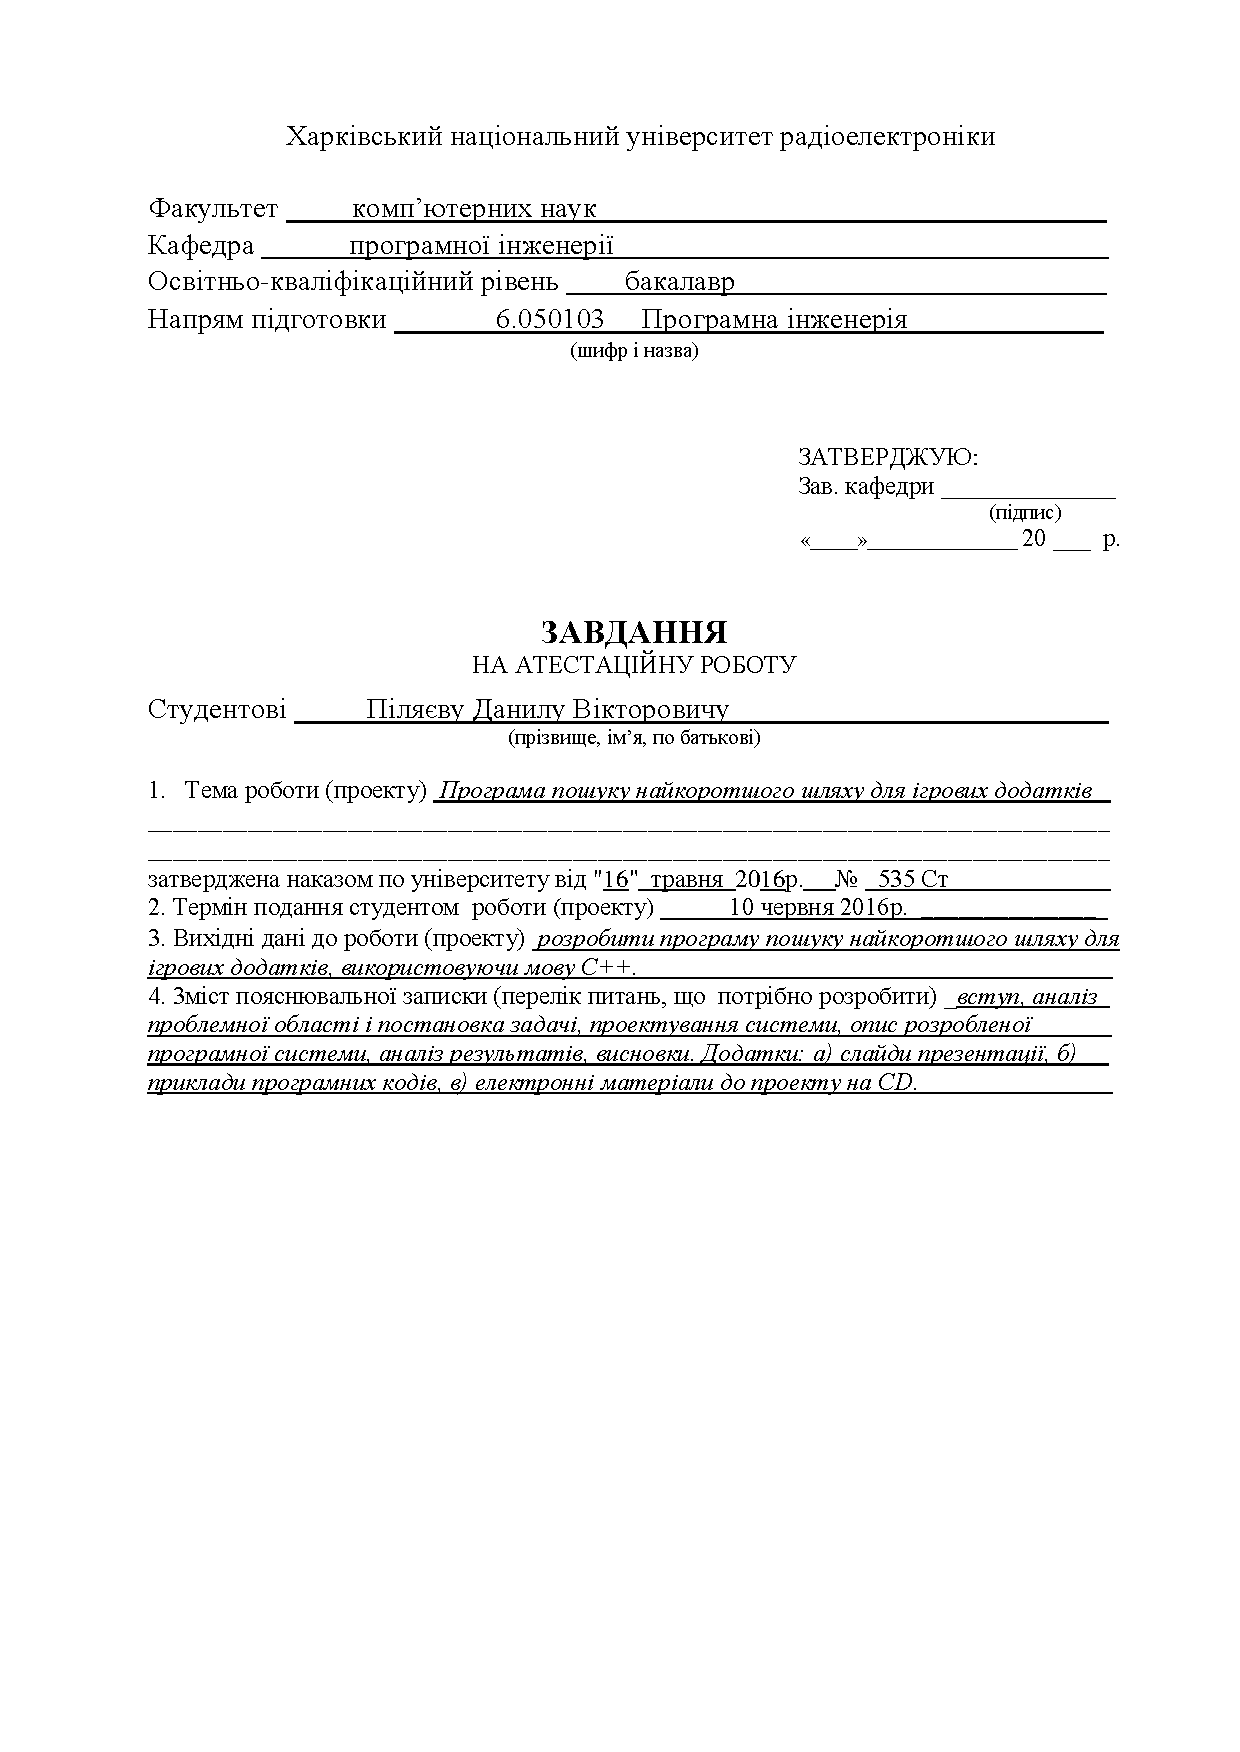
\includepdf[pages=1-2]{task_new.pdf}

\section*{РЕФЕРАТ}

\vspace{1\baselineskip}

\thispagestyle{empty}

Звіт з переддипломної практики бакалаврів: \pageref{LastPage} сторінок, \totalsections\ розділів,  \totalfigures\ рисунків, 8 джерел, 1 додаток.

Об'єкт проектування -- бібліотека для пошуку путей шляхів.

Метою роботи є створення оптимізованної бібліотеки для пошуку шляхів в игрових додатків.

Методи розробки базуються на язиці С++11, та бібліотеках threadpool11, SFML і SFGUI

У результаті роботи була здійснена програмна реалізація бібліотеки для пошуку путей шляхів в игрових додатків, а саме алгоритмів A*, JPS та Goal Bounding. В процессі ці алгоритми були проаналізовані та оптимізовані.

БИБЛИОТЕКА, ПОИСК ПУТЕЙ, C++, A*, JPS, GOAL BOUNDING, HAA*, КВАДРАТНАЯ СЕТКА, ЭВРИСТИЧЕСКАЯ ФУНКЦИЯ.

\vspace{1\baselineskip}

Explanatory note: \pageref{LastPage} pages, \totalsections\ sections,  \totalfigures\ figures, 8 sources, 1 application.

Subject of architecturing -- library for path finding.

The aim is to create optimized library for path finding in games.

The development methods are based on С++11 and libraries threadpool11, SFML and SFGUI.

The result of work is implemented library for path finding in games which includes A* and JPS algorithms. During development this algorithms were analyzed and optimized.

LIBRARY, ПPATH FINDING, C++, A*, JPS, GOAL BOUNDING, HAA*, SQUARE GRID, HEURISTIC FUNCTION.

\clearpage

\section*{СОДЕРЖАНИЕ}

\thispagestyle{empty}

\setlength{\cftbeforesecskip}{0pt}
\renewcommand{\cftsecpagefont}{\normalfont}

\renewcommand{\cfttoctitlefont}{\hspace{0.38\textwidth} \MakeUppercase}
\renewcommand{\cftbeforetoctitleskip}{-1em}
\renewcommand{\cftsecfont}{\hspace{31pt}}
\renewcommand{\cftsubsecfont}{\hspace{11pt}}

\renewcommand{\cftparskip}{-1mm}
\renewcommand{\cftdotsep}{1}
\setcounter{tocdepth}{2} 
\renewcommand*\contentsname{}
\thispagestyle{empty}

\tableofcontents

\thispagestyle{empty}
    
\clearpage

\section*{ВВЕДЕНИЕ}
\addcontentsline{toc}{section}{Введение}

\vspace{1\baselineskip} 

Задачей нахождения кратчайшего пути является поиск оптимального и короткого пути между двумя точками. Проблема нахождения кратчайших путей возникает в таких случаях как: оптимизация перевозки грузов и пассажиров, оптимальная маршрутиризация пакетов в сети, навигация искусственного интеллекта и игрока в компьютерных играх, а так же навигация роботов в пространстве. Все компьютерные игры имеют поиск путей в том или ином виде, поэтому скорость и точность алгоритма часто влияет на качество искусственного интеллекта и восприятия игрока. 

Существует несколько представлений пространства для проведения поиска путей, одним из них является квадратная сетка, которая проста для создания и используется в стратегиях реального времени и других играх с двумерной картой. Хотя квадратная сетка в большинстве случаев является неоптимальным представлением области поиск, с ней очень просто работать и легко модифицировать, что значительно упрощает программную работу с игровой картой. В следствии неоптимальности представления карты появляется необходимость в оптимизации алгоритмов поиска работающих с ней посредством общей оптимизации логики работы алгоритма, введение некоторых допущений и ограничений на область поиска, а так же проведение низкоуровневых оптимизаций.

Таким образом, задача нахождения кратчайшего пути на области представленной квадратной сеткой является актуальной проблемой, которая будет рассмотрена и исследована в данной работе.

Целью преддипломной практики является проведение анализа существующих алгоритмов поиска путей, разработка различных вариантов алгоритмов и их оптимизаций, создание оптимизированной универсальной библиотеки для нахождения оптимальных маршрутов и анализ полученных результатов.



\clearpage

%\section[Организационная структура предприятия]{ОРГАНИЗАЦИОННАЯ СТРУКТУРА ПРЕДПРИЯТИЯ}

\vspace{1\baselineskip} 
Программа пошуку нойкоротшого шляху для игрових додаткив
Харьковский национальный университет радиоэлектроники — ХНУРЭ.
В университете обучается более 12 тысяч студентов по 34 специальностям. ХНУРЭ включает 9 факультетов, и 30 кафедр. 

Преддипломная практика проходила на базе кафедры программной инженерии (ПИ). В состав кафедры входят четыре научные лаборатории.

 Кафедра программной инженерии является профилирующей при подготовке бакалавров по направлению «Программная инженерия» (ПИ), магистров и специалистов по специальности «Инженерия программного обеспечения» (ИПО), «Программное обеспечение систем» (ПОС). Стандарт образования по направлению «программная инженерия» полностью отвечает европейскому стандарту «Software Engineering».

Кафедра программной инженерии сотрудничает в сфере обучения и науки в IT с Институтом математики и системной инженерии (School of Mathematics and Systems Engineering) в Швеции.

На базе научных лабораторий, лаборатории Бизнес-Инкубатор и учебно-научного отряда "Программист" организовываются семинары и кружки в рамках которых студенты имеют возможность повысить свой профессиональный уровень.
%
%\clearpage

\section[Анализ предметной области]{\MakeTextUppercase{АНАЛИЗ ПРЕДМЕТНОЙ ОБЛАСТИ}}
\vspace{-1\baselineskip} 
\subsection{Алгоритмы нахождения кратчайших путей}

Задачей нахождения кратчайшего пути является поиск оптимального и короткого пути между двумя точками. Решения этой задачи в большинстве случаев основаны на алгоритме Дейкстры \cite{Dijkstra} для нахождения кратчайшего пути во взвешенных графах. 

Простейшие алгоритмы для обхода графа, такие как поиск в ширину и поиск в глубину могут найти какой-то путь от начальной до конечной вершины, но не учитывают стоимость пути. Одним из первых алгоритмов поиска пути с учётом его стоимости был алгоритм Беллмана -- Форда, который проходит по всем возможным маршрутам и находит наиболее оптимальный, вследствие чего имеет временную сложность $O(|V||E|)$, где $V$ - количество вершин, а $E$ - количество рёбер. Однако для нахождения пути близкого к оптимальному не обязательно перебирать все пути, а можно отсекать неперспективные направления на основе некой эвристики, что может дать таким алгоритмам нижнюю оценку $O(|E|\log(|V|))$. Такими алгоритмами являются алгоритм Дейкстры, A* и их модификации.

\subsubsection{A*}

Алгоритм A{*} (A звёздочка) - это алгоритм общего назначения, который может быть использован для решения многих задач, например для нахождения путей. A{*} является вариацией алгоритма Дейкстры и используя эвристическую функция для ускорения работы, при этом гарантируя наиболее эффектное использование онной \cite{A_STAR}. 

Алгоритм A{*} поочерёдно рассматривает наиболее перспективные неисследованные точки или точки с неоптимальным маршрутом до них, выбирая пути которые минимизируют $ f(n) = g(n) + h(n) $, где $n$ последняя точка в пути, $g(n)$ - стоимость пути от начальной точки до точки $n$, а $h(n)$ - эвристическая оценка стоимости пути от $n$ до конца пути. Когда точка исследована, алгоритм останавливается если это конечная точка, иначе все её соседи добавляются в список для дальнейшего исследования.

Для нахождения пути от начальной до конечной точки, кроме стоимости пути до точки, следует записывать и её предка (точку из которой мы пришли в неё).

%\begin{algorithm}
%    \caption{Псевдокод A*}\label{alg:a-star-example}
%    \begin{algorithmic}[1]
%        \State Добавляем начальную точку в открытый список.
%        \Repeat
%        \State Поиск точки из открытого списка с наименьшим значением функции f.
%        \State Добавить точку в закрытый список.
%        \ForAll{точек соседних текущей}
%        \If{точка входит в закрытый список}
%        \State Игнорировать её.
%        \ElsIf{точка не в открытом списке}
%        \State Добавляем точку в открытый список. 
%        \State Делаем текущую точку предком этой точки. 
%        \State Подсчитываем её параметры.
%        \Else
%        \If{возможно ли улучшить длину пути через неё} 
%        \State Меняем её предка и пересчитываем параметры.
%        \EndIf
%        \EndIf
%        \EndFor
%        \Until Конечная точка не добавлена в закрытый список и открытый список не пуст.
%    \end{algorithmic}
%\end{algorithm}

Свойства алгоритма A*:

\begin{enumerate}
    \item Алгоритм гарантирует нахождение пути между точками, если он существует;
    \item Если эвристическая функция $h(n)$ не переоценивает действительную минимальную стоимость пути, то алгоритм работает наиболее оптимально;
    \item A* оптимально эффективен для заданной эвристики $h(n)$.
\end{enumerate}

На оценку сложности A* влияет использованная эвристика, в худшем случае количество точек рассмотренных A* экспоненциально растёт по сравнению с длинной пути, однако при эвристике $h(n)$ удовлетворяющей условию $|h(x) - h^*(x)| \leq O(\log h^*(x))$, где $h^*(n)$ - оптимальная эвристика, алгоритм будет иметь полиномиальную сложность. Так же на временную сложность влияет выбранный способ хранения закрытых и открытых точек.

\subsubsection{JPS}

Jump Point Search (JPS) - эффективная техника для нахождения и отброса симметричных путей \cite{IMPROVING_JPS}. JPS представляет собой модификацию алгоритма A* с двумя правилами отброса точек. Применения этих правил позволяет увеличить производительность поиска путей на квадратной сетки на порядок - без препроцессинга и дополнительной памяти.

JPS действует в предположении, что прохождение по клеткам карты намного быстрее добавления их в открытые и закрытые списки. При этом одна клетка может рассматриваться много раз в течении одного поиска.

В JPS существует два набора правил: правила отброса клеток и правила прыжков.

Имея клетку $x$, достижимую из родительской клетки $p$, мы отбрасываем из соседей $x$ любую клетку $n$ для которой исполняется хотя бы одно из условий:

\begin{enumerate}
	\item существует путь от $p$ до $n$ равный $\pi'=(p,x,n)$ строго короче чем путь от $p$ до $n$ через клетку $x$ равный $\pi=(p,x,n)$;
	\item существует путь от $p$ до $n$ равный $\pi'=(p,n)$ такой же длины как путь от $p$ до $n$ через клетку $x$ равный $\pi=(p,x,n)$, но путь $\pi'$ имеет диагональное перемещение раньше чем путь $\pi$. 
\end{enumerate}

Для вычисления каждого из правил достаточно проверки только соседей данной точки.  

Преимуществами JPS является отсутствие препроцессинга, дополнительного потребления памяти, постоянное ускорение A* на порядок. Главным недостатком является, то что он работает только на картах с одинаковой стоимостью прохода по клеткам, однако существует теоретическое решение данной проблемы, но любое её решение приводит к уменьшение преимущества JPS над простым A*.

\subsubsection{HPA* и HAA*}

HPA* (Hierarchical Path-Finding A*) - добавляет алгоритму A* иерархическую абстракцию, разбивая карту на прилегающие друг к другу кластеры, которые соединены входами \cite{HPA}. Одной из основных идей алгоритма является то, что расчёт пути в A* каждый раз происходит с нуля, что можно исправить добавив сохранение кратчайших путей между определёнными точками. 

Первым этапом алгоритма является препроцессинг карты для построения кластеров и их входов. При этом возможно построение нескольких уровней графа кластеров используя один и тот же алгоритм рекурсивно на созданных во время предыдущего прохода кластерах.

Во время исполнения программы запрос нахождения пути выполняется рекурсивно находя и уточняя путь на графе начиная с самых крупного уровня кластеров. После нахождения пути может применятся его сглаживание.


Алгоритм HPA* работает с такими допущениями:

\begin{enumerate}
    \item Все актёры имеют одинаковый размер, при этом все части навигационной сетки проходимы ими;
    \item На всех участках карты агенты имеют одинаковую проходимость.
\end{enumerate}

Иерархическая структура карты сильно ускоряет поиск пути, однако алгоритм HPA* работает не учитывая такие важные параметры как размер агентов и проходимость местности.  

В итоге размер агентов и проходимость карты должны учитываться при нахождении пути, что в случае с алгоритмом HPA* приводит к тому, что эти параметры должны учитываться при оценки путей между входами.

Алгоритм иерархического поиска является достаточно абстрактным для учёта указанных проблем. Для этого на основе алгоритма HPA* был создан алгоритм HAA* (Hierarchical Annotated A*), который при создании путей между входами кластера учитывает размеры актёров и проходимость местности.

Основная разница с алгоритмом HPA* у алгоритма HAA* состоит в шаге формирования пути между транзитными точками в рамках кластера и дальнейшем шаге их оптимизации. При нахождении пути между транзитными точками в кластере следует найти пути для всех агентов разных размеров и проходимости 

В итоге алгоритм HAA* имеет такие же преимущества как HPA*, а так же возможность учёта размера агента и проходимости карты. В зависимости от выбранной тактики устранения похожих путей между транзитными точками кластеров конечный путь будет хуже оптимального до 4-8\%.


\subsection{Различные представления области поиска}

Для поиска пути требуется некоторое представление области поиска, от его выбора зависит скорость работы алгоритма, точность его работы и качество пути. Так же выбор способа представления влияет на занимаемое областью место в оперативной памяти. 

Глобально пространства поиска можно разделить на дискретные и непрерывные, далее будут рассматриваться только дискретные пространства (для непрерывных пространств существуют алгоритмы сведения их к дискретным).  

Можно выделить такие способы представления: квадратная сетка, quadtree (дерево квадрантов), navmesh (навигационная сетка), waypoints (путевые точки).

\subsubsection{Квадратная сетка}

Квадратная сетка является самым простым и очевидным представлением области поиска. Подходит для игр жанра TD (tower defence) и некоторых RTS игр. 

Обладает такими преимуществами: проста в использовании и представлении в памяти, можно быстро и легко добавлять и удалять препятствия, легко поддерживать различную проходимость карты и различные размеры агентов. 

К недостаткам можно отнести большое занимаемое в памяти место, сложность поддержки многоуровневых карт а так же наименьшую скорость работы алгоритма A* с данным представлением. 

Некоторые алгоритмы поиска путей не работают на других представлениях кроме квадратной сетки, например JPS.

\subsubsection{Quadtree (дерево квадрантов)}

Дерево квадрантов является усовершенствованной версией квадратной сетки. Позволяет сильно уменьшить занимаемое место за счёт объединения одинаковых участков, так же позволяет ускорить алгоритм поиска пути. Минусом можно считать усложнение добавления и удаления элементов из карты.

\subsubsection{Navmesh (навигационная сетка)}

Навигационная сетка - набор выпуклых многоугольников, которые описывают проходимую часть трёхмерного мира. 

Является популярной техникой для описания трёхмерных карт. Навигационная сетка часто автоматически генерируется из трёхмерного мира, однако при этом возникает проблема оптимизации числа полигонов для ускорения работы поиска путей и уменьшении веса сетки.

Преимуществами навигационной сетки являются: возможность представить многоуровневый мир, низкое потребление памяти, скорость поиска пути, точность. Недостатком является сложность динамического изменения мира.

\subsubsection{Waypoints (путевые точки)}

Путевые точки - набор точек и рёбер по которым можно ходить. Обычно создаются вручную.

Преимущества: просты в использовании, возможно описать пути любой сложности ( в воздухе, в воде и т.д.), простота изменения, гибкость работы.

Недостатки: медленней чем навигационная сетка, пути выходят хуже (более длинные и неестественные).

\subsection{Эвристические функции}

Эвристическая функция $h(n)$ вычисляет для алгоритмов поиска путей основанных на A* приблизительную стоимость маршрута от точки до цели. Эвристика может использоваться для контролирования поведения алгоритмов \cite{HEURISTICS}:

\begin{enumerate}
	\item если $h(n)$ равно нулю, то A* вырождается алгоритм Дейкстры;
	\item если $h(n)$ всегда меньше или равен стоимости пути от точки до цели, то A* гарантирует нахождение кратчайшего пути, однако чем больше разница между $h(n)$ и реальной стоимостью, тем больше точек раскрывает алгоритм и тем медленней работает;
	\item если $h(n)$ равен стоимости пути от точки до цели, то A* следует только по оптимальному пути, что делает его очень быстрым, однако такая эвристика невозможна в общих случаях;
	\item если $h(n)$ переоценивает стоимость пути, то A* не гарантирует нахождение кратчайшего пути, однако это может ускорить его;
	\item если $h(n)$ очень сильно переоценивает стоимость пути, то алгоритм вырождается в жадный.
\end{enumerate}

Исходя из этого можно сделать вывод, что при выборе эвристики осуществляется выбор между скоростью и точностью.

Что бы получить эвристику, которая всегда равна стоимости от точки до цели, нужно предрасчитать пути между каждыми парами точек, что не осуществимо на реальных картах. Однако существует некоторые упрощения и модификации этой эвристики:

\begin{enumerate}
	\item покрыть карту более крупной сеткой и уже для неё рассчитывать данную эвристику;
	\item выделить некоторые путевые точки и рассчитывать эвристику между ними;
	\item сохранять не все расстояния от точки до остальных, а только по одной области для каждого направления, содержащие все точки до которых оптимальный путь идёт в выбранном направлении (Goal Bounding).
\end{enumerate}

Для различных представлений области поиска существуют разные эвристики. Для области представленной квадратной сеткой можно выделить такие эвристики:

\begin{enumerate}
	\item расстояние городских кварталов (Manhattan distance) - расстояние равное сумме модулей разностей координат точек $|x_1 - x_2| + |y_1-y_2|$;
	\item евклидова метрика (Euclidean distance) - равна расстоянию между точками вычисленному по теореме пифагора $\sqrt{(x_1 - x_2)^2 + (y_1 - y_2)^2}$;
	\item эвристики препятствующие прохождению по путям с одинаковой стоимостью (Tie breaaking).
\end{enumerate} 

\subsection{Goal Bounding}

Goal Bounding - техника отброса заранее неподходящих точек, которая позволяет значительно ускорить поиск пути \cite{GOAL_BOUNDING}. Goal Bounding можно разделить на два этапа:

\begin{enumerate}
	\item оффлайн этап - представляет собой препроцессинг карты с целью найти и сохранить прямоугольники для каждого из направлений, ограничивающие минимальную область на карте, которая включает в себя все точки карты до которых путь через выбранное направление является самым оптимальным.
	\item онлайн этап - прекращение итераций в выбранном направлении если целевая точка не входит в его ограничивающий прямоугольник.
\end{enumerate}
 
Данная техника применима для всех областей поиска и для всех алгоритмов поиска. Её недостатком является время препроцессинга и занимаемое место результирующими данными. Препроцессинг работает за $O(n^2)$, где $n$ - количество узлов на карте, что делает невозможным пересчёт во время исполнения программы. Количество занимаемой памяти - линейно и для квадратной сетки с 8 направлениями равно $ 4 * 32 * n$ байт.

Этап препроцессинга легко поддаётся распараллеливанию, что позволяет работать даже с большими картами, имея достаточное количество вычислительной мощности.  

\subsection{Выбор алгоритма и представления области поиска}

Выбор алгоритма сильно зависит от выбранного типа области поиска, в данной аттестационной работе была выбрана область поиска представленная квадратной сеткой. Нахождения пути на ней является самым затратным по производительности, поэтому оптимизация алгоритмов работающих с этим представлением является актуальной задачей. 

Как базовый алгоритм был взят A*. По сравнению с JPS алгоритмы HPA* и HAA*, работают дольше и являются намного сложнее в реализации, которая может быть несоразмерна с полученной от них выгодой, однако они могут выдавать начальные участки пути намного быстрее чем JPS и A*, что в некоторых случаях оправдывает их написание. В данной работе был выбран алгоритм JPS.  


\subsection{Постановка задачи}

Целью аттестационной работы является проведение анализа существующих алгоритмов поиска путей, разработка различных вариантов алгоритмов и их оптимизаций, создание оптимизированной универсальной библиотеки для нахождения оптимальных маршрутов в контексте игровых приложений и анализ полученных результатов. 

Создание библиотеки состоит из заданий:

\begin{enumerate}
    \item анализ алгоритмов нахождения путей;
    \item разработка алгоритма A*;
    \item разработка алгоритма JPS;
    \item разработка препроцессинга Goal Bounding;
    \item интеграция Goal Bounding в алгоритм A*;
    \item интеграция Goal Bounding в алгоритм JPS;
    \item разработка удобного визуализатора для наглядной оценки и проверки алгоритмов;
    \item создание модуля для сравнения и валидации алгоритмов.
\end{enumerate}

Для написания библиотеки был выбран язык C++. Для визуализации результатов была выбрана библиотека SFML и SFGUI. Для написания параллельных алгоритмов - библиотека threadpool11, которая реализует пул потоков.

\clearpage

\section[Проектирование программного обеспечения]{\MakeTextUppercase{ПРОЕКТИРОВАНИЕ ПРОГРАММНОГО ОБЕСПЕЧЕНИЯ}}
\vspace{-1\baselineskip} 
\subsection{Программное обеспечение}

Для написание библиотеки нахождения кратчайших путей был выбран язык программирования C++ стандарта C++11. С++ является современным языком высокого уровня, который предоставляет широкие возможности по оптимизации кода, в отличии от интерпретируемых языков и языков с JIT оптимизациями. Так же С++ широко используется в игровых приложениях. Для создания библиотеки язык С++ был выбран по следующим причинам: кроссплатформенность, быстродействие, возможность низкоуровневых оптимизаций, простота внедрения библиотеки в существующие программные продукты. 

Стандарт C++11 привнёс в язык многие функции, которые позволяют писать более понятный и современный код, уменьшить количество случайных ошибок и повысить читаемость. В следствии чего были устранены многие недостатки в сравнении с другими языками программирования.

В C++11 для измерения времени используется стандартная библиотека chrono. В chrono существует несколько реализаций измерения времени:

\begin{enumerate}
    \item system\_clock -- общесистемное время;
    \item steady\_clock -- монотонное время, которое никогда не подстраивается;
    \item high\_resolution\_clock - наиболее точное время с наименьшим доступным периодом.  
\end{enumerate} 

Для измерения времени была выбрана реализация high\_resolution\_clock.

Библиотека SFML (Simple and Fast Multimedia Library) -- кроссплатформенная библиотека для создания мультимедийных приложений. Имеет простой платформонезависимый интерфейс для рисования графики.

SFGUI - библиотека работающая совместно с библиотекой SFML и предоставляющая возможности для отрисовывания интерфейсов.

Для использования многопоточности была подключена библиотека threadpool11, которая реализует пул потоков \cite{THREAD_POOL}.

Для написания кода библиотеки была выбрана среда разработки CLion, которая имеет редактор с поддержкой синтаксиса C++11 и его подсветкой, имеет средства рефакторинга и поддерживает различные CVS, например Git. Так же имеется поддержка CMake -- системы кроссплатформенной сборки проектов, управления зависимостями и тестами.

В качестве системы контроля версий был выбран Git. Git -- распределённая система контроля версий, которая направлена на скорость работа и целостность данных, имеет гибкую и простую систему создания и объединения веток. Репозиторий проекта был размещён на удалённом сервисе BitBucket.
%
%\subsection{Архитектура ПО}

\subsection{UML-моделирование ПО}

Унифицированный язык моделирования (UML) -- язык общего назначения для визуализации, спецификации, конструирования и документации программных систем \cite{UML_USER_GUIDE_2ND}. Язык UML объединяет в себе семейство разных графических нотаций с общей метамоделью. 

Преимуществами UML являются:

\begin{enumerate}
    \item объектно-ориентированность, что делает его близким к современным объектного-ориентированным языкам;
    \item расширяем, что позволяет вводить собственные текстовые и графические стереотипы;
    \item прост для чтения;
    \item позволяет описать системы со всех точек зрения.
\end{enumerate}

В UML используется три вида диаграмм:

\begin{enumerate}
    \item структурные диаграммы -- отражают статическую структуру системы;
    \item диаграммы поведения -- отражают поведение системы в динамике, показывают, что должно происходить в системе;
    \item диаграммы взаимодействия -- подвид диаграмм поведения, которые выражают передачу контроля и данных внутри системы.
\end{enumerate} 

Для моделирования системы проектируемой в данной аттестационной работе будут использованы структурная и поведенческая диаграммы, а именно диаграмма классов (Class diagram) и диаграмма вариантов использования (Use case diagram).

Диаграмма классов является статическим отображением системы, которая демонстрирует её классы, их аттрибуты, методы и взаимосвязи. Диаграмма классов является прямым отображением классов присутствующих в системе.

Диаграмма состоит из классов и связей между ними. В свою очередь классы состоят из имени класса, его полей и методов. Поля и методы могут иметь модификаторы доступа к ним: публичный -- знак плюс, приватный -- знак минус, защищённый -- решётка и некоторые другие. Методы могут иметь аргументы и возвращаемое значение и их типы.

Связи между классами делятся на связи между созданными объектами класса и на связи на уровне самих классов. Связи между объектами включают в себя:

\begin{enumerate}
	\item зависимость -- односторонняя зависимость между двумя классами, когда изменения в одном влияют на второй;
	\item ассоциация -- набор схожих связей, которые обозначают, что один объект выполняет некоторые действия над другим, такие как: вызов метода или посылка сообщения;
	\item агрегация -- включение одним классом другого, однако при этом их жизненные циклы не зависимы;
	\item композиция -- включение одним классом другого, при этом существует зависимость между жизненным циклом контейнера и включаемого класса.
\end{enumerate}

Связи между классами делятся на:

\begin{enumerate}
	\item обобщение -- обозначает, что один из двух классов является подклассом второго;
	\item реализация -- обозначает, что класс реализует поведение определённое во втором.
\end{enumerate}

В разрабатываемой библиотеки можно выделить центральный интерфейс, который является основным интерфейсом для взаимодействия с ней, это PathFinder \cref{fig:diagram_classes}. Он является шаблонным классом и параметризуется типом координат (целочисленный тип), он имеет один метод -- Find, который принимает начальную позицию, конечную позицию и тип актёра (проходимость актёра), а возвращает вектор клеток являющихся найденным маршрутом. Его реализуют классы SimpleAStar и JPSAstar, которые в свою очередь имеют следующие шаблонные параметры: тип карты, эвристика, включение Goal Bounding и включение режима отладки.  

\addimg{path_finding_classes.png}{1.1}{Диаграмма классов}{diagram_classes}

Интерфейс для реализации эвристика, Heuristic, содержит метод nodes\_distance, который принимает текущую точку, конечную точку и начальную точку, а возвращает приближённо оценённую стоимость маршрута от текущей до конечной точки. Эвристика включается в PathFinder как шаблонный класс.

Класс GoalBounding реализует одноимённый алгоритм и содержит методы для препроцессинга карты с заданным типом актёра, для загрузки и сохранения информации полученный при препроцессинге, а так же для отброса направлений при поиске пути. Данный класс включается в класс карты и используется в классах реализующих PathFinder.

Класс карты является базовой реализацией карты и содержит методы для получение данных о препроцессинге, размеров картыб проверки вхождения точки в область карты и метод получения клетки карты. Класс карты передаётся в PathFinder через конструктор и хранится в нём. Карта включает в отдельные клетки MapNode, которые имеют вес, проходимость и метод для проверки на проходимость.

Карта загружается по средством класса MapLoader, который имеет единственный метод для загрузки карты по её имени.

Диаграмма вариантов использования позволяет отразить представленную систему в динамике, а именно собрать требования к системе отражающие внешние и внутренние воздействия. Она позволяет показать взаимодействие различных пользователей и частей системы. Целями диаграммы вариантов являются:

\begin{enumerate}
	\item сбор требований к системе;
	\item получение вида системы со стороны;
	\item идентификация внутренних и внешних воздействий на систему;
	\item показ взаимодействия требований и актёров.
\end{enumerate}

Диаграмма вариантов использования состоит из вариантов использования, которые представляют собой некоторую высокоуровневую функцию системы определённую через анализ требований, актёров, которые являются чем-то, что взаимодействует с системой и связей между вариантами использования и актёрами \cite{USE_CASE}.

Актёром может быть как человек или организация, которая использует систему, так и внешний сервис взаимодействующий с ней. Графически актёр обычно представляется в виде человечка.

Взаимодействие актёра и варианта использования отражается посредством стрелки между ними.

При создании варианта использования стоит уделять внимание выбору его имени. Оно должно чётко определять выполняемую функцию и начинаться с глагола. 

Варианты использования могут включать другие и расширять их. Варианты использования создаются и рисуются от самых крупных уровней к самым мелким.

В разрабатываемой библиотеки можно выделить программиста, который использует её, как актёра. В свою очередь как варианты использования можно выделить части упрощённого интерфейса библиотеки \cref{fig:diagram_use_case}, что даёт нам три варианта использования: 

\begin{enumerate}
	\item ``Выполнить препроцессинг'' карты;
	\item ``Найти путь'', который реализован двумя разными алгоритмами и может быть расширен с помощью Goal Bounding алгоритма;
	\item ``Загрузить карту'', который реализован в виде загрузки простой текстовой карты.
\end{enumerate}

\addimg{path_finding_use_case.png}{0.75}{Диаграмма Use case}{diagram_use_case}

\subsection{Требования к ПО}

Библиотека должна предоставлять интерфейс для нахождения путей различными алгоритмами с поддержкой:

\begin{enumerate}
    \item одного универсального интерфейса для всех алгоритмов; 
	\item различных реализаций карт;
	\item различных эвристик;
	\item включения и выключения Goal Bounding алгоритма;
	\item возможностью опционально получить информацию для отладки алгоритмов.
\end{enumerate}

Должен иметься интерфейс для работы с Goal Bounding алгоритмом включающий в себя: препроцессинг карты, сохранение и загрузка результатов.

Так же библиотека должна предоставлять базовую реализацию карты и её загрузчика.

Библиотека должна зависить только от стандартной библиотеки и библиотеки threadpool11.

Библиотека не должна включать платформозависимый код и в следствии чего должна компилироваться на различных платформах, таких как: x32, x86-64, arm.

Библиотека должна иметь простой способ включения в другие проекты.   

\subsection{Описание интерфейса взаимодействия с библиотекой}

Для работы с библиотекой требуется её включение в проект по средством CMake или её подключение в бинарном виде. 

CMake - расширяемая система с открытым исходным кодом, которая управляет процессом сборки не зависимо от целевого компилятора. В отличии от других кроссплатформных систем, CMake работает совместно с родными для компиляторов окружениями сборки. В следствии чего CMake генерирует стандартные файлы для сборки для каждого конкретного компилятора.
Так же CMake имеет гибкую систему настроек, что позволяет создавать множество целей сборки, которые могут зависить от разных условий, например платформы на которой происходит компиляция.

Основным интерфейсом взаимодействия с библиотекой является интерфейс нахождения путей PathFinder<CoordsType> \cref{fig:path_finding_interface}, который имеет метод find с аргументами начальной, конечной точки и типа актёра (его проходимость), а возвращать массив точек представляющих собой найденный маршрут.

\begin{figure}[!htb]
	\centering
	\captionsetup{justification=centering}
	\begin{lstlisting}
template<class CoordsType>
class PathFinder
{
public:
virtual std::vector<Point<CoordsType>> find( CoordsType startX, 
					CoordsType startY,
					CoordsType targetX,
					CoordsType targetY,
					uint32_t unitType ) = 0;
};
	\end{lstlisting}
	\caption{Интерфейс нахождения путей}
	\label{fig:path_finding_interface}
\end{figure}

Так же предоставляется интерфейс для модификации работы алгоритмов (типа карты, эвристики, Goal Bounding) посредством шаблонов. Из-за того, что количество параметров шаблонов большое, библиотекой предоставляется несколько предзаданных вариантов.

Библиотекой предоставляется интерфейс и реализация базовой версии карты, который включает в себя загрузку карты, получение её параметров и отдельных клеток, а так же выполнение препроцессинга Goal Bounding.   


\clearpage

\section[Описание программной реализации]{\MakeTextUppercase{ОПИСАНИЕ ПРОГРАММНОЙ РЕАЛИЗАЦИИ}}

\vspace{1\baselineskip} 

При реализации библиотеки и визуализатора возникли задачи не связанные с реализацией самих алгоритмов, такие как: корректное измерение времени работы алгоритмов и включение отдельных методов в зависимости от типа с которым работает они работают.

Для корректного измерение времени был создан класс MeasureUtils, который включает в себя методы для измерения скорости работы обычных функций и методов классов. Данные методы являются шаблонными, что позволяет добиться их универсальности. Они принимают настройки тестирования, которые содержат количество вызовов функции для прогрева и количество вызовов для измерения скорости, так же передаётся сама функция и её аргументы. Прогрев нужен что бы данные и инструкции гарантировано оказались в кэше процессора, чем уменьшили влияние времени на пересылку данных из оперативной памяти и кэшей нижнего уровня. Время выполнения функции равно общему времени её выполнения в цикле поделённому на количество итераций в цикле.

Включение и выключение методов в данной работе требуется для работы со знаковы и беззнаковыми целыми типами - для беззнаковых типов не требуется проверка на то, является ли переменная отрицательной, что нужно для проверки находится ли точка в границах карты. Данная проблемы решена двумя макросами  ``PF\_FUN\_ENABLE\_IF\_SIGNED'' и ``PF\_FUN\_ENABLE\_IF\_UNSIGNED'' \cref{fig:enable_fun_macro}.

\begin{figure}[!htb]
	\centering
	\captionsetup{justification=centering}
	\begin{lstlisting}
#define PF_FUN_ENABLE_IF_SIGNED( ValueType, ReturnType ) \
template<class Q = ValueType> \
enable_if_t<std::is_integral<Q>::value &&  std::is_signed<Q>::value, ReturnType>

#define PF_FUN_ENABLE_IF_UNSIGNED( ValueType, ReturnType ) \
template<class Q = ValueType> \
enable_if_t<std::is_integral<Q>::value &&  std::is_unsigned<Q>::value, ReturnType>
	\end{lstlisting}
	\caption{Макросы для включения методов}
	\label{fig:enable_fun_macro}
\end{figure}

\subsection{Реализации алгоритма A*}

Алгоритм A* является базовым и наиболее часто используемым алгоритмом для поиска путей. Для работы алгоритм использует открытый и закрытый список. В открытый список добавляется начальная точка, открытый список содержит точки, которые мы уже нашли, но ещё не рассмотрели. После чего пока в открытом списке существуют точки -- выбирается точка с наименьшей стоимостью и рассматриваются её соседи. Если стоимость пути через данную точку до соседа меньше записанной в него стоимости, то стоимость пути до него изменяется и его родитель меняется на текущую клетку \cref{fig:a_star_open_list_add}. После рассмотрения точки - она добавляется в закрытый список. Если открытый список оказался пуст -- значит пути до конечной точки не существует. Если из открытого списка была взята конечная точка - это означает, что путь существует и можно реконструировать его. Для этого мы берём родителя конечной точки и рекурсивно рассматриваем её родителей в массив, пока не дойдём до начальной точки \cref{fig:a_star_reconstruct_path}.

\begin{figure}[!htb]
	\centering
	\captionsetup{justification=centering}
	\begin{lstlisting}
NodeInfo& nextNodeInfo = m_nodesInfo[nextNodeIdx];
if( !nextNodeInfo.IsVisited() || newCost < nextNodeInfo.GetNodeCost())
{
	nextNodeInfo.SetVisited( true );
	nextNodeInfo.SetNodeCost( newCost );
	nextNodeInfo.SetCameFrom( best.x, best.y );
	float priority =
		newCost +
		Heuritic::nodes_distance( nextX, nextY, targetX, targetY, startX, startY );
	openList.push( PriorityNode<CoordsType>( nextX, nextY, priority ));
}
	\end{lstlisting}
	\caption{Добавление в открытый список в A*}
	\label{fig:a_star_open_list_add}
\end{figure}

\begin{figure}[!htb]
	\centering
	\captionsetup{justification=centering}
	\begin{lstlisting}
std::vector<Point<CoordsType>> path;
auto current = Point<CoordsType>( targetX, targetY );
path.push_back( current );
while( !current.Equals( startPoint ))
{
	auto nodeIdx = coords_to_contiguous_idx( current.x, current.y, m_map.GetSizeX());
	const auto& info = m_nodesInfo[nodeIdx];
	if( current == info.GetCameFrom())
	{
		break;
	}
	
	current = info.GetCameFrom();
	path.push_back( current );
}
	\end{lstlisting}
	\caption{Реконструкция пути}
	\label{fig:a_star_reconstruct_path}
\end{figure}

При написании A* для открытого списка была использована очередь с приоритетом std::priority\_queue, а для закрытого списка -- вектор имеющий размер карты. Такая реализация закрытого списка дала возможность делать проверку на вхождение в него за константное время. Память для закрытого списка выделяется один раз при создании экземпляра алгоритма поиска и при каждом поиске у всех клеток сбрасывается флаг посещённости.

\subsection{Реализация алгоритма JPS}

Алгоритм JPS представляет собой усовершенствование алгоритма A*. Недостатком A* является то, что он добавляет в открытый список все клетки, которые являются прямыми соседями рассматриваемой и имеют больший вес чем вес текущая клетка плюс стоимость пути между ними, JPS в свою очередь предоставляет возможность пропуска добавления многих клеток на основе возможной симметрии путей. Множество симметричных путей возникает на отрытых пространствах. Пути называются симметричными, потому что они практически идентичны. Алгоритм A* не учитывает возможность симметричности путей, тогда как JPS использует её вводя некоторые допущения о карте для увеличения производительности поиска. 

Для пропуска добавления лишних клеток вводятся функции прыжков, которые делятся на горизонтальные, вертикальные и диагональные.

Логика работы горизонтального и вертикального прыжка одинакова. Рассмотрим горизонтальный прыжок право -- остальные варианты происходят по аналогии с ним. При этом мы можем сделать следующие допущения \cite{JPS_DETAILS}:

\begin{enumerate}
    \item клетка из который мы пришли может быть проигнорирована;
    \item клетки по диагонали позади рассматриваемой, мы тоже можем игнорировать, так как они были достигнуты из родительской клетки \cref{fig:jps_cells_ignored_behind};
    \item клетки выше и ниже рассматриваемой могут быть достигнуты оптимальнее из её родителя \cref{fig:jps_cells_ignored_up_down};
    \item клетки правее и выше/ниже рассматриваемой могут быть достигнуты оптимальнее из клеток на одну левее;
\end{enumerate}

\addtikz{Отброшенные клетки сзади}{jps_cells_ignored_behind}{1}
{
\mybox[x=1,y=0,color=grey]
\mybox[x=1,y=1,color=grey]
\mybox[x=1,y=2,color=grey]
\mybox[x=2,y=1,color=green]

\mygrid[width=6, height=3]

\myarrow[startx=0,starty=1,endx=1,endy=1,color=darkgrey]
\myarrow[startx=1,starty=1,endx=2,endy=1,color=darkgrey]
\myarrow[startx=1,starty=1,endx=1,endy=2,color=blue]
\myarrow[startx=1,starty=1,endx=1,endy=0,color=blue]
}

\addtikz{Отброшенные клетки сверху и снизу}{jps_cells_ignored_up_down}{1}
{
	\mybox[x=1,y=0,color=grey]
	\mybox[x=1,y=1,color=grey]
	\mybox[x=1,y=2,color=grey]
	\mybox[x=2,y=0,color=grey]
	\mybox[x=2,y=2,color=grey]
	\mybox[x=2,y=1,color=green]
	
	\mygrid[width=6, height=3]
	
	\myarrow[startx=0,starty=1,endx=1,endy=1,color=darkgrey]
	\myarrow[startx=1,starty=1,endx=2,endy=1,color=darkgrey]
	\myarrow[startx=1,starty=1,endx=1,endy=2,color=darkgrey]
	\myarrow[startx=1,starty=1,endx=1,endy=0,color=darkgrey]
	\myarrow[startx=1,starty=1,endx=2,endy=2,color=blue]
	\myarrow[startx=1,starty=1,endx=2,endy=0,color=blue]
}

Эти допущения приводят к тому что алгоритм должен рассматривать только клетки правее от текущий пока путь не содержит препятствий \cref{fig:jps_forward_move}. Однако путь не всегда свободен от препятствий, что ломает приведённой допущение. Это происходит в том случае, когда клетка сверху или снизу рассматриваемой является препятствием, что делает утверждение о том, что оптимальный путь до диагональной клетки не проходит через рассматриваемую \cref{fig:jps_horizontal_forced_neighbour}. В такой ситуации прыжок останавливается и клетка по диагонали (такая клетка называется вынужденным соседом) и текущая клетка добавляются в открытый список для дальнейшего рассмотрения. 

Последним допущением является то, что если при прыжке препятствие блокирует продвижение в заданном направлении - весь прыжок может быть отброшен \cref{fig:jps_forward_move_blocked}.

\addtikz{Отброшенные клетки сверху и снизу}{jps_forward_move}{1}
{
	\mybox[x=1,y=0,color=grey]
	\mybox[x=1,y=1,color=grey]
	\mybox[x=1,y=2,color=grey]
	\mybox[x=2,y=0,color=grey]
	\mybox[x=2,y=2,color=grey]
	\mybox[x=2,y=0,color=grey]
	\mybox[x=2,y=2,color=grey]
	\mybox[x=3,y=0,color=grey]
	\mybox[x=3,y=2,color=grey]
	\mybox[x=4,y=0,color=grey]
	\mybox[x=4,y=2,color=grey]
	\mybox[x=2,y=1,color=green]
	
	\mygrid[width=6, height=3]
	
	\myarrow[startx=0,starty=1,endx=1,endy=1,color=darkgrey]
	\myarrow[startx=1,starty=1,endx=2,endy=1,color=darkgrey]
	\myarrow[startx=1,starty=1,endx=1,endy=2,color=darkgrey]
	\myarrow[startx=1,starty=1,endx=1,endy=0,color=darkgrey]
	\myarrow[startx=1,starty=1,endx=2,endy=2,color=darkgrey]
	\myarrow[startx=1,starty=1,endx=2,endy=0,color=darkgrey]
	\myarrow[startx=2,starty=0,endx=3,endy=0,color=darkgrey]
	\myarrow[startx=2,starty=2,endx=3,endy=2,color=darkgrey]
	\myarrow[startx=3,starty=0,endx=4,endy=0,color=darkgrey]
	\myarrow[startx=3,starty=2,endx=4,endy=2,color=darkgrey]
	\myarrow[startx=2,starty=1,endx=3,endy=1,color=blue]
	\myarrow[startx=3,starty=1,endx=4,endy=1,color=blue]
}

\addtikz{Вынужденный сосед}{jps_horizontal_forced_neighbour}{1}
{
	\begin{scope}[]
		\matrix[column sep=1cm, ampersand replacement=\&]{
			\mybox[x=1,y=0,color=grey]
			\mybox[x=1,y=1,color=grey]
			\mybox[x=1,y=2,color=grey]
			\mybox[x=2,y=0,color=grey]
			\mybox[x=2,y=2,color=black]
			\mybox[x=3,y=2,color=red]
			\mybox[x=3,y=0,color=grey]
			\mybox[x=2,y=1,color=green]
			
			\mygrid[width=6, height=3]
			
			\myarrow[startx=0,starty=1,endx=1,endy=1,color=darkgrey]
			\myarrow[startx=1,starty=1,endx=2,endy=1,color=darkgrey]
			\myarrow[startx=1,starty=1,endx=1,endy=2,color=darkgrey]
			\myarrow[startx=1,starty=1,endx=1,endy=0,color=darkgrey]
			\myarrow[startx=1,starty=1,endx=2,endy=2,color=red]
			\myarrow[startx=1,starty=1,endx=2,endy=0,color=darkgrey]
			\myarrow[startx=2,starty=0,endx=3,endy=0,color=darkgrey]
			\myarrow[startx=2,starty=1,endx=3,endy=2,color=blue]
			\myarrow[startx=2,starty=1,endx=3,endy=1,color=blue];
			
			\&
			
			\mybox[x=1,y=0,color=grey]
			\mybox[x=1,y=1,color=grey]
			\mybox[x=1,y=2,color=grey]
			\mybox[x=2,y=0,color=black]
			\mybox[x=2,y=2,color=grey]
			\mybox[x=3,y=2,color=grey]
			\mybox[x=3,y=0,color=red]
			\mybox[x=2,y=1,color=green]
			
			\mygrid[width=6, height=3]
			
			\myarrow[startx=0,starty=1,endx=1,endy=1,color=darkgrey]
			\myarrow[startx=1,starty=1,endx=2,endy=1,color=darkgrey]
			\myarrow[startx=1,starty=1,endx=1,endy=2,color=darkgrey]
			\myarrow[startx=1,starty=1,endx=1,endy=0,color=darkgrey]
			\myarrow[startx=1,starty=1,endx=2,endy=2,color=darkgrey]
			\myarrow[startx=2,starty=2,endx=3,endy=2,color=darkgrey]
			\myarrow[startx=1,starty=1,endx=2,endy=0,color=red]
			\myarrow[startx=2,starty=1,endx=3,endy=0,color=blue]
			\myarrow[startx=2,starty=1,endx=3,endy=1,color=blue];
			\\
		};
	\end{scope}
}

\addtikz{Заблокированный путь}{jps_forward_move_blocked}{1}
{
	\mybox[x=1,y=0,color=grey]
	\mybox[x=1,y=1,color=grey]
	\mybox[x=1,y=2,color=grey]
	\mybox[x=2,y=0,color=grey]
	\mybox[x=2,y=2,color=grey]
	\mybox[x=2,y=0,color=grey]
	\mybox[x=2,y=2,color=grey]
	\mybox[x=3,y=0,color=grey]
	\mybox[x=3,y=2,color=grey]
	\mybox[x=4,y=0,color=grey]
	\mybox[x=4,y=2,color=grey]
	\mybox[x=2,y=1,color=green]
	\mybox[x=5,y=1,color=black]
		
	\mygrid[width=6, height=3]
	
	\myarrow[startx=0,starty=1,endx=1,endy=1,color=darkgrey]
	\myarrow[startx=1,starty=1,endx=2,endy=1,color=darkgrey]
	\myarrow[startx=1,starty=1,endx=1,endy=2,color=darkgrey]
	\myarrow[startx=1,starty=1,endx=1,endy=0,color=darkgrey]
	\myarrow[startx=1,starty=1,endx=2,endy=2,color=darkgrey]
	\myarrow[startx=1,starty=1,endx=2,endy=0,color=darkgrey]
	\myarrow[startx=2,starty=0,endx=3,endy=0,color=darkgrey]
	\myarrow[startx=2,starty=2,endx=3,endy=2,color=darkgrey]
	\myarrow[startx=3,starty=0,endx=4,endy=0,color=darkgrey]
	\myarrow[startx=3,starty=2,endx=4,endy=2,color=darkgrey]
	\myarrow[startx=2,starty=1,endx=3,endy=1,color=blue]
	\myarrow[startx=3,starty=1,endx=4,endy=1,color=blue]
}

Такие же правила и допущения верны для диагональных прыжков. Рассмотрим прыжок вправо вверх по диагонали, можно предположить, что клетки снизу, снизу справа, слева и слева сверху можно оптимально достичь через родителя рассматриваемой клетки. В следствии  чего остаётся рассмотреть три клетки: сверху, справа и по диагонали \cref{fig:jps_diagonal_jump}. В отличии от горизонтального и вертикального прыжка в данном случае осталось три клетки для рассмотрения, однако для двух из них требуется вертикальный и горизонтальный прыжок. Так как требуемые прыжки уже определены -- вначале происходят они, затем если в результате прыжков не было найдено клеток для дальнейшего рассмотрения -- происходит прыжок по диагонали на одну клетку и процесс повторяется.

\addtikz{Прыжок по диагонали}{jps_diagonal_jump}{1}
{
	\mybox[x=1,y=1,color=grey]
	\mybox[x=1,y=2,color=grey]
	\mybox[x=1,y=3,color=grey]
	\mybox[x=2,y=1,color=grey]
	\mybox[x=3,y=1,color=grey]
	\mybox[x=2,y=2,color=green]
	
	\mygrid[width=5, height=5]
	
	\myarrow[startx=0,starty=0,endx=1,endy=1,color=darkgrey]
	\myarrow[startx=1,starty=1,endx=1,endy=2,color=darkgrey]
	\myarrow[startx=1,starty=2,endx=1,endy=3,color=darkgrey]
	\myarrow[startx=1,starty=1,endx=2,endy=1,color=darkgrey]
	\myarrow[startx=2,starty=1,endx=3,endy=1,color=darkgrey]
	\myarrow[startx=1,starty=1,endx=2,endy=2,color=darkgrey]
	\myarrow[startx=2,starty=2,endx=2,endy=3,color=blue]
	\myarrow[startx=2,starty=2,endx=3,endy=2,color=blue]
	\myarrow[startx=2,starty=2,endx=3,endy=3,color=blue]
}

По аналогии с горизонтальным и вертикальным прыжком при диагональном прыжке так же встречаются вынужденные соседи, когда слева или под текущей клеткой находится препятствие, клетка слева вверху или справа внизу соответственно являются вынужденными соседями \cref{fig:jps_diagonal_jump_forced_neighbour}. 

\addtikz{Вынужденный сосед при диагональном прыжке}{jps_diagonal_jump_forced_neighbour}{1}
{
	\begin{scope}[]
		\matrix[column sep=1cm, ampersand replacement=\&]{
			% % % % % % % % % %
			\mybox[x=1,y=1,color=grey]
			\mybox[x=1,y=2,color=grey]
			\mybox[x=1,y=3,color=grey]
			\mybox[x=2,y=1,color=black]
			\mybox[x=3,y=1,color=red]
			\mybox[x=2,y=2,color=green]
			
			\mygrid[width=5, height=5]
			
			\myarrow[startx=0,starty=0,endx=1,endy=1,color=darkgrey]
			\myarrow[startx=1,starty=1,endx=1,endy=2,color=darkgrey]
			\myarrow[startx=1,starty=2,endx=1,endy=3,color=darkgrey]
			\myarrow[startx=1,starty=1,endx=2,endy=1,color=red]
			\myarrow[startx=2,starty=2,endx=3,endy=1,color=blue]
			\myarrow[startx=1,starty=1,endx=2,endy=2,color=darkgrey]
			\myarrow[startx=2,starty=2,endx=2,endy=3,color=blue]
			\myarrow[startx=2,starty=2,endx=3,endy=2,color=blue]
			\myarrow[startx=2,starty=2,endx=3,endy=3,color=blue]; 
			
			\& % % % % % % % %
			
			\mybox[x=1,y=1,color=grey]
			\mybox[x=1,y=2,color=black]
			\mybox[x=1,y=3,color=red]
			\mybox[x=2,y=1,color=grey]
			\mybox[x=3,y=1,color=grey]
			\mybox[x=2,y=2,color=green]
			
			\mygrid[width=5, height=5]
			
			\myarrow[startx=0,starty=0,endx=1,endy=1,color=darkgrey]
			\myarrow[startx=1,starty=1,endx=1,endy=2,color=red]
			\myarrow[startx=2,starty=2,endx=1,endy=3,color=blue]
			\myarrow[startx=1,starty=1,endx=2,endy=1,color=darkgrey]
			\myarrow[startx=2,starty=1,endx=3,endy=1,color=darkgrey]
			\myarrow[startx=1,starty=1,endx=2,endy=2,color=darkgrey]
			\myarrow[startx=2,starty=2,endx=2,endy=3,color=blue]
			\myarrow[startx=2,starty=2,endx=3,endy=2,color=blue]
			\myarrow[startx=2,starty=2,endx=3,endy=3,color=blue]; 
			\\
	};
	\end{scope}
}

Когда прыжок закончен берётся клетка с наименьшим весом из открытого списка и из неё происходит прыжок в направлении в котором алгоритм пришёл в неё.

JPS начинается с того, что из начальной точки происходят прыжки во все восемь сторон. Затем выполняется цикл по открытому списку и если в нём существует клетка, то из неё происходит вертикальный и горизонтальный прыжок, затем выполняется проверка не допускающая прохождение между двумя непроходимыми клетками. После чего запускается диагональный прыжок. 

Диагональный прыжок происходит пока следующая клетка проходима, не является конечной клеткой и находится на карте. Пусть текущая клетка имеет координаты ${(x_c, y_c)}$, а направлением прыжка является пара дельт ${(d_x, d_y)}$ принимающих значения ${d_x, d_y \in \{-1, 0, 1\}}$. Сперва рассматривается соседняя клетка ${(x_c, y_c+d_y)}$ и если она проходима и соседняя  ${(x_c-d_x, y_c)}$ не проходима, а клетка с координатами ${(x_c-d_x, y_c+d_y)}$ проходима (путь не заблокирован \cref{fig:jps_diagonal_jump_blocked_forced_neighbour}), то текущая клетка проверяется на возможность добавления в открытый список. Такая же проверка происходит с тройкой точек ${\{(x_c+d_x), (x_c, y_c-d_y), (x_c+d_x, y_c-d_y)\}}$ соответственно. Если прыжок вперёд заблокирован двумя клетками по горизонтали и вертикали ${\{(x_c, y_c+d_y), (x_c+d_x, y_c)\}}$ \cref{fig:jps_blocked_diagonal_jump}, то прыжок прекращается, иначе проводится горизонтальный и вертикальный прыжок и если хотя бы один из них нашёл клетку для дальнейшего рассмотрения, то текущая клетка добавляется в открытый список, при этом такие прыжки в стороны не добавляют клетки в открытый список.
  
\addtikz{Заблокированный вынужденный сосед}{jps_diagonal_jump_blocked_forced_neighbour}{1}
{
	\mybox[x=1,y=1,color=grey]
	\mybox[x=1,y=2,color=grey]
	\mybox[x=1,y=3,color=grey]
	\mybox[x=2,y=1,color=black]
	\mybox[x=3,y=2,color=black]
	\mybox[x=3,y=1,color=yellow]
	\mybox[x=2,y=2,color=green]
	
	\mygrid[width=5, height=5]
	
	\myarrow[startx=0,starty=0,endx=1,endy=1,color=darkgrey]
	\myarrow[startx=1,starty=1,endx=1,endy=2,color=darkgrey]
	\myarrow[startx=1,starty=2,endx=1,endy=3,color=darkgrey]
	\myarrow[startx=2,starty=2,endx=2,endy=3,color=blue]
	\myarrow[startx=1,starty=1,endx=2,endy=2,color=darkgrey]
	\myarrow[startx=2,starty=2,endx=3,endy=2,color=red]
	\myarrow[startx=2,starty=2,endx=3,endy=1,color=red]
	\myarrow[startx=2,starty=2,endx=3,endy=3,color=blue]
}
  
\addtikz{Заблокированный прыжок по диагонали}{jps_blocked_diagonal_jump}{1}
{
	\mybox[x=1,y=1,color=grey]
	\mybox[x=1,y=2,color=grey]
	\mybox[x=1,y=3,color=grey]
	\mybox[x=2,y=1,color=grey]
	\mybox[x=3,y=1,color=grey]
	\mybox[x=3,y=1,color=grey]
	\mybox[x=2,y=3,color=black]
	\mybox[x=3,y=2,color=black]
	\mybox[x=2,y=2,color=green]
	
	\mygrid[width=5, height=5]
	
	\myarrow[startx=0,starty=0,endx=1,endy=1,color=darkgrey]
	\myarrow[startx=1,starty=1,endx=1,endy=2,color=darkgrey]
	\myarrow[startx=1,starty=2,endx=1,endy=3,color=darkgrey]
	\myarrow[startx=1,starty=1,endx=2,endy=1,color=darkgrey]
	\myarrow[startx=2,starty=1,endx=3,endy=1,color=darkgrey]
	\myarrow[startx=1,starty=1,endx=2,endy=2,color=darkgrey]
	\myarrow[startx=2,starty=2,endx=2,endy=3,color=red]
	\myarrow[startx=2,starty=2,endx=3,endy=2,color=red]
	\myarrow[startx=2,starty=2,endx=3,endy=3,color=red]
}
  
Горизонтальный и вертикальный прыжки происходят пока следующая клетка проходима, не является конечной клеткой и находится на карте. На каждом шаге происходит проверка на наличие вынужденных соседей и если такой сосед найден, то он добавляется в открытый список и метод прерывается. 

Когда открытый список исчерпан -- происходит восстановление пути так же как и в A*.

\subsection{Реализация и интеграция GoalBounds}

Алгоритм Goal Bounding можно разделить на два этапа: этап препроцессинга и проверка направления во время выполнения поиска пути. Во время препроцессинга происходит прохождение по всем клеткам карты, для каждой клетки выполняет волновой алгоритм, который заполняет все клетки стоимостью путей до них от начальной клетки и изначальным направлением по которому алгоритм пришёл в данную клетку. После чего для данной клетки определяется 8 ограничивающих прямоугольников \cref{fig:goal_bounding_dbg}, по одному на каждое направление \cref{fig:goal_bounding_fill}. Определяются они по такому алгоритму: 

\begin{enumerate}
	\item делаем минимальную точку прямоугольника равную координатам правой верхней точки карты, а максимальную - равной левой нижней;
	\item идём по всем точкам и расширяем прямоугольник соответствующий направлению в котором точка была достигнута из начальной, что бы прямоугольник включал её. 
\end{enumerate}

\begin{figure}[!htb]
	\centering
	\captionsetup{justification=centering}
	\begin{lstlisting}
auto& bbNode = m_bbMap.GetNodeBB( startX, startY );
for( uint16_t i = 0; i < map.GetSizeX(); i++ )
{
	for( uint16_t j = 0; j < map.GetSizeY(); j++ )
	{
		 auto& ffNode = ffMap->GetNode( i, j ); 
		 if( map.IsPassable( i, j, type ))
		 {
			 auto& dirBB = bbNode.boundingBoxes[static_cast<int>(ffNode.originalDir)];	 
			 dirBB.minX = std::min( dirBB.minX, i );
			 dirBB.maxX = std::max( dirBB.maxX, i );
			 dirBB.minY = std::min( dirBB.minY, j );
			 dirBB.maxY = std::max( dirBB.maxY, j );
		 }
	 }
 }
	\end{lstlisting}
	\caption{Определение ограничивающих прямоугольников}
	\label{fig:goal_bounding_fill}
\end{figure}

\addimg{img/goal_bounding_dbg.png}{0.8}{Часть карты с раскрашенными в разные цвета ограничивающими прямоугольниками}{goal_bounding_dbg}

Так как алгоритм вычисляет ограничивающие прямоугольники для каждой клетки независимо, то его можно распараллелить. Для этого был использован пул поток, реализованный библиотекой threadpool11. Для каждой клетки создаётся своя задача и добавляется в очередь, после добавления всех задач происходит ожидание их завершения. Каждый поток имеет свою карту для волнового алгоритма которая создаётся один раз для одного потока. После исполнения алгоритма результат записывается в файл рядом с файлом карты, в файле поочерёдно, для каждой клетки, записано 32 целочисленных значения -- четыре значения для каждого из восьми направлений из клетки, которые являются верхней левой и правой нижней точкой прямоугольника. Если файл с результатами вычислений уже существует на диске, то загружается он, что бы не проводить трудоёмкие вычисления заново.

Для включения Goal Bounding в A* требуется добавить проверку на правильность направления сразу после проверки на вхождение точки в границу карты при циклическом обходе соседей текущей точки \cref{fig:a_star_test_goal_bounds}. 

\begin{figure}[!htb]
	\centering
	\captionsetup{justification=centering}
	\begin{lstlisting}
for( int i = 0; i < 8; i++ )
{
	const auto& delta = coordDeltas[i];
	const CoordsType nextX = best.x + delta.first;
	const CoordsType nextY = best.y + delta.second;
	if( m_map.IsNodeOnMap( nextX, nextY ))
	{
		if( TestGoalBounding( best.x, best.y, targetX, targetY, dirs[i] ))
		{
			const MapNode& node = m_map.GetNode( nextX, nextY );
			if( node.IsPassable( unitType ))
			{
	\end{lstlisting}
	\caption{Проверка Goal Bounds}
	\label{fig:a_star_test_goal_bounds}
\end{figure}

Для добавления Goal Bouding в JPS требуется провести аналогичное действие, но для всех функций прыжков.

\subsection{Реализация визуализатора}

Для реализации визуализатора были использованы кроссплатформенные библиотеки SFML и SFGUI. Карта рисуется несколькими слоями, которые для удобства и скорости отрисовываются в отдельные текстуры. Визуализатор рисует такие слои: слой карты, последний найденный путь, открытые клетки алгоритмом A*, направления прыжков алгоритма JPS, ограничивающие прямоугольники алгоритма Goal Bounding для выбранной клетки.

Нахождение пути происходит после выбора начальной и конечной точки, после чего он отображается на карте и выводится приблизительное время выполнения алгоритма. 

Визуализатор, кроме отображения путей с отладочной информацией имеет возможность сравнивать скорость выполнения алгоритмов для выбранного пути.

\subsection{Реализация сравнения алгоритмов}

Для сравнения алгоритмов поиска пути был создан отдельный программный модуль. Данный модуль позволяет проводить измерение времени выполнения алгоритмов на различных сценариях. Выбранным форматом сценариев стал формат использующийся для сценариев расположенных на сайте ``movingai.com/benchmarks/''. 

Каждый файл с сценарием содержит набор различных тестов, обычно сгруппированных по картам. Каждый тест содержит путь к карте, ширину и высоту карты, координаты начальной, координаты конечной точки и ожидаемую стоимость пути. Сценарии представлены текстовыми файлами с тестами разделёнными новой строкой.

Программа сравнения алгоритмов имеет такие этапы:

\begin{enumerate}
	\item считывание сценариев из указанной папки;
	\item считывание пройденных тестов;
	\item загрузка карт указанных в сценариях;
	\item определение параметров выполнения тестов;
	\item удаление тестов для которых не была найдена карты или которые уже были пройдены;
	\item сортировка тестов по размеру карты;
	\item вычисление Goal Bounding;
	\item проведение тестов для карты;
	\item запись результатов тестов в csv файл.
\end{enumerate}   

Результатом выполнения программы является csv файл в который записаны результаты выполнения всех тестов из найденных сценариев. После прерывания выполнения программы при последующем запуске тесты начнутся с последнего прерванного, что позволяет проводить тесты в несколько сессий.

Каждая запись в результатах содержит имя карты, размерность карты, название протестированного алгоритма, количество вызовов алгоритма, среднее время выполнения одного вызова, общее время выполнения, результирующую стоимость пути, координаты начальной и конечной точки.  

Для ускорения выполнения тестов существует возможность выполнять их в несколько потоков, однако при увеличении количества потоков может понижаться точность измерений.

Данный программный модуль так же является средством для тестирования корректности работы алгоритмов, так как производит большое число тестов на разных картах.

\clearpage

\section[Анализ результатов]{\MakeTextUppercase{АНАЛИЗ РЕЗУЛЬТАТОВ}}

\subsection{Сравнительный анализ алгоритмов}

Сравнительный анализ алгоритмов проводился на картах из таких игр: ``Dragon Age: Origins'', ``Warcraft III'', ``Baldurs Gate II ''. Для выполнения анализа были взяты карты и пути с сайта ``movingai.com/benchmarks/'', где собраны подготовленные наборы данных состоящие из карт и сценариев к ним. В ходе сравнительного анализа было использовано 267 различных карт: 36 из ``Warcraft III'', 156 из ``Dragon Age: Origins'' и 75 из ``Baldurs Gate II ''. Количество протестированных путей в общей сложности составило 1070000. Для Astar и JPS без модификации Goal Bounding было протестировано больше путей чем с данной модификацией, так как карты с размерностью более 512 на 512 были исключены из препроцессинга. На карты с большим размером время препроцессинга оказывалось очень большим.

Тестирование алгоритмов проводилось на компьютере со следующими характеристиками: процессором AMD FX-8320 с частотой 3.5 ghz и оперативной памятью 16gb DDR3 1333 mhz. Программа выполнялась под операционной системой Windows 10 без каких-либо запущенных сторонних процессов. Программа для тестирования была скомпилирована с ключом O3 компилятором g++ версии 5.3.  

В ходе анализа алгоритмов было получено более миллиона уникальных векторов данных, которые первоначально экспортились в формат csv, однако для последующего анализа они были импортированы в реляционную базу данных PostgreSQL, что сильно упростило манипуляцию с данными.

Рассмотрим результаты выполнения алгоритмов на карте AR0011SR размером 512 на 512 \cref{fig:a_star_alg_cmp_AR0011SR}.

\addtikz{Сравнение алгоритмов на карте AR0011SR}{a_star_alg_cmp_AR0011SR}{1}
{
	\begin{axis}[
		name=plot1,
		xlabel={Стоимость пути},
		ylabel={миллисекунды},
		ymode=log,
		log ticks with fixed point,
		legend pos=outer north east]
		\addplot[smooth,mark=*,black] plot coordinates {
			(0,0.450337827586206897 )
			(30,0.473905788888888889)
			(60,0.526151056179775281)
			(90,0.603534767676767677)
			(120,0.859617405063291139)
			(150,1.0536403333333333  )
			(180,1.3990839574468085  )
			(210,2.2270172111111111  )
			(240,2.3663113736263736  )
			(270,3.01304575          )
			(300,3.848451175         )
			(330,4.4758353296703297  )
			(360,5.6996502413793103  )
			(390,6.27858416          )
			(420,7.6057240178571429  )
			(450,8.6096742142857143  )
		};
		\addplot[smooth,mark=square*,black] plot coordinates {
			(0,0.446724137931034483  )
			(30,0.446576022222222222 )
			(60,0.457549224719101124 )
			(90,0.491480683673469388 )
			(120,0.5109110625        )
			(150,0.529025333333333333)
			(180,0.593930297872340426)
			(210,0.651347263736263736)
			(240,0.724399197802197802)
			(270,0.8862859           )
			(300,0.928384075949367089)
			(330,0.858660098901098901)
			(360,0.995955793103448276)
			(390,1.0348355866666667)
			(420,1.251526363636364 )
			(450,1.8444414666666667)
		};
		\addplot[dotted,mark=*,mark options={solid},black] plot coordinates {
			(0,0.012311942857142857  )
			(30,0.015875864197530864 )
			(60,0.01732458904109589  )
			(90,0.01950175           )
			(120,0.023366141025641026)
			(150,0.025258567567567568)
			(180,0.027953415584415584)
			(210,0.029131767123287671)
			(240,0.036167641975308642)
			(270,0.038806767123287671)
			(300,0.04332785          )
			(330,0.048559086956521739)
			(360,0.049925911392405063)
			(390,0.054420759036144578)
			(420,0.0565024           )
			(450,0.050475512195121951)
			(480,0.07050855)
			(510,0.084748  )
		};
		\addplot[dashed,mark=square*,mark options={solid},black] plot coordinates {
			(0,0.055721971428571429  )
			(30,0.068408641975308642 )
			(60,0.09245564           )
			(90,0.097469831168831169 )
			(120,0.117343753246753247)
			(150,0.148138506849315068)
			(180,0.146065987341772152)
			(210,0.153351256756756757)
			(240,0.209265075949367089)
			(270,0.234806376623376623)
			(300,0.267204269230769231)
			(330,0.323374849315068493)
			(360,0.364171797297297297)
			(390,0.502699630952380952)
			(420,0.533060150684931507)
			(450,0.622631926829268293)
			(480,0.704095943396226415)
			(510,0.639205)
		};
		\legend{A*,A*+GB,JPS+GB,JPS}
	\end{axis} 	
}

 Самой быстрой является комбинация алгоритма JPS и Goal Bounding, при этом время выполнения одного вызова варьировалось от 12 до 80 микросекунд. Время выполнения JPS варьировалось от 55 до 700 микросекунд, что в 3-10 раз хуже чем с Goal Bounding \cref{fig:a_star_relation_path_to_call_time}. A* с и без Goal Bounding на коротких путях показывают примерно одинаковое время. На длинных путях модификация Goal Bounding даёт преимущество в несколько раз (в 3-5 раз). Время выполнения A* доходит до 9 миллисекунд, что для игровых приложений очень долго, так как это время близко ко времени полной отрисовки кадра, а найти может потребоваться больше одного пути.

\addtikz{Зависимость длительности одного вызова поиска пути от его стоимости для карты AR0011SR (512x512)}{a_star_relation_path_to_call_time}{1}
{
			\begin{axis}[
				name=plot1,
				xlabel={Стоимость пути},
				ylabel={миллисекунды},
				legend pos=north west]
				\addplot[smooth,mark=*,black] plot coordinates {
			(0,0.450337827586206897 )
			(30,0.473905788888888889)
			(60,0.526151056179775281)
			(90,0.603534767676767677)
			(120,0.859617405063291139)
			(150,1.0536403333333333  )
			(180,1.3990839574468085  )
			(210,2.2270172111111111  )
			(240,2.3663113736263736  )
			(270,3.01304575          )
			(300,3.848451175         )
			(330,4.4758353296703297  )
			(360,5.6996502413793103  )
			(390,6.27858416          )
			(420,7.6057240178571429  )
			(450,8.6096742142857143  )
				};
				\legend{A*}
			\end{axis}
			
				\begin{axis}[
					name=plot3,
					at=(plot1.below south east), anchor=above north east,
					xlabel={Стоимость пути},
					ylabel={миллисекунды},
					legend pos=north west]
					\addplot[smooth,mark=*,black] plot coordinates {
			(0,0.446724137931034483  )
			(30,0.446576022222222222 )
			(60,0.457549224719101124 )
			(90,0.491480683673469388 )
			(120,0.5109110625        )
			(150,0.529025333333333333)
			(180,0.593930297872340426)
			(210,0.651347263736263736)
			(240,0.724399197802197802)
			(270,0.8862859           )
			(300,0.928384075949367089)
			(330,0.858660098901098901)
			(360,0.995955793103448276)
			(390,1.0348355866666667)
			(420,1.251526363636364 )
			(450,1.8444414666666667)
					};
					\legend{A*+GB}
				\end{axis} 
			
			
			\begin{axis}[
				name=plot4,
				at=(plot3.right of north east), anchor=left of north west,
				xlabel={Стоимость пути},
				ylabel={микросекунды},
				ytick scale label code/.code={},
				scaled y ticks=base 10:3,
				legend pos=north west]
				\addplot[smooth,mark=*,black] plot coordinates {
			(0,0.012311942857142857  )
			(30,0.015875864197530864 )
			(60,0.01732458904109589  )
			(90,0.01950175           )
			(120,0.023366141025641026)
			(150,0.025258567567567568)
			(180,0.027953415584415584)
			(210,0.029131767123287671)
			(240,0.036167641975308642)
			(270,0.038806767123287671)
			(300,0.04332785          )
			(330,0.048559086956521739)
			(360,0.049925911392405063)
			(390,0.054420759036144578)
			(420,0.0565024           )
			(450,0.050475512195121951)
			(480,0.07050855)
			(510,0.084748  )
				};
				\legend{JPS+GB}
			\end{axis} 
			
			\begin{axis}[
				name=plot2,
				at=(plot4.above north west), anchor=below south west,
				xlabel={Стоимость пути},
				ylabel={микросекунды},
				ytick scale label code/.code={},
				scaled y ticks=base 10:3,
				legend pos=north west]
				\addplot[smooth,mark=*,black] plot coordinates {
			(0,0.055721971428571429  )
			(30,0.068408641975308642 )
			(60,0.09245564           )
			(90,0.097469831168831169 )
			(120,0.117343753246753247)
			(150,0.148138506849315068)
			(180,0.146065987341772152)
			(210,0.153351256756756757)
			(240,0.209265075949367089)
			(270,0.234806376623376623)
			(300,0.267204269230769231)
			(330,0.323374849315068493)
			(360,0.364171797297297297)
			(390,0.502699630952380952)
			(420,0.533060150684931507)
			(450,0.622631926829268293)
			(480,0.704095943396226415)
			(510,0.639205)
				};
				\legend{JPS}
			\end{axis} 

}

На разных картах алгоритмы могут вести себя по разному \cref{fig:a_star_alg_cmp_brc501d}. В случае карты brc501d алгоритм JPS в большинстве случаев медленней чем комбинация A* и Goal Bounding, хотя всё равно остаётся намного быстрей обычного A*. В данном случае карта имеет такое строение, что многие пути имеют вид ``крюков'' огибающих очень длинное препятствие, в таком случае алгоритм JPS сканирует очень много клеток и хотя в открытый список добавляются немногие из них, большое количество клеток проходится безрезультатно. На рисунке \ref{fig:jps_degradation} показан такой случай - непроходимые клетки обозначены чёрным цветом, красная ломаная показывает найденный путь, а сине-зелёные полоски показывают направления в которых проходил алгоритм JPS. Как можно заметить для нахождения пути алгоритму пришлось пройти всю карту больше одного раза.

\addtikz{Сравнение алгоритмов на карте brc501d}{a_star_alg_cmp_brc501d}{1}
{
	\begin{axis}[
		name=plot1,
		xlabel={Стоимость пути},
		ylabel={миллисекунды},
		ymode=log,
		log ticks with fixed point,
		legend pos=outer north east]
		\addplot[smooth,mark=*,black] plot coordinates {
			(0,0.052029395348837209 )
			(30,0.085476139534883721)
			(60,0.185111410526315789)
			(90,0.453184678571428571)
			(120,0.857330337078651685)
			(150,1.2929210119047619  )
			(180,1.7794124285714286  )
			(210,2.179155            )
			(240,2.9767070625        )
			(270,3.4637211012658228  )
			(300,4.4178079117647059  )
			(330,4.6648257654320988  )
			(360,5.8247307653061224  )
			(390,5.8970600810810811  )
			(420,5.9309958255813953  )
			(450,5.8462961219512195  )
			(480,6.5784044444444444  )
		};
		\addplot[smooth,mark=square*,black] plot coordinates {
			(0,0.046492755813953488  )
			(30,0.056089627906976744 )
			(60,0.068674452631578947 )
			(90,0.085188905882352941 )
			(120,0.100951609195402299)
			(150,0.106980767441860465)
			(180,0.152424012048192771)
			(210,0.201235827586206897)
			(240,0.2231119375        )
			(270,0.326703936708860759)
			(300,0.341250617647058824)
			(330,0.400953475         )
			(360,0.570358858585858586)
			(390,0.525511561643835616)
			(420,0.379954482352941176)
			(450,0.522641047619047619)
			(480,1.1540081111111111)			
		};
		\addplot[dotted,mark=*,mark options={solid},black] plot coordinates {
			(0,0.00695063157894736842)
			(30,0.00875052           )
			(60,0.010565513157894737 )
			(90,0.0143075            )
			(120,0.016939310810810811)
			(150,0.019650253164556962)
			(180,0.023864923076923077)
			(210,0.025602753246753247)
			(240,0.029741623376623377)
			(270,0.036766671428571429)
			(300,0.038822779220779221)
			(330,0.053536639534883721)
			(360,0.07151592          )
			(390,0.082788410256410256)
			(420,0.09895061038961039 )
			(450,0.101980703703703704)
			(480,0.102642347222222222)
			(510,0.1125517)	
		};
		\addplot[dashed,mark=square*,mark options={solid},black] plot coordinates {
			(0,0.022047896103896104  )
			(30,0.02765783950617284  )
			(60,0.037216481012658228 )
			(90,0.073302469879518072 )
			(120,0.102604518987341772)
			(150,0.139790822784810127)
			(180,0.243236886075949367)
			(210,0.337014340909090909)
			(240,0.467919648648648649)
			(270,0.809973689189189189)
			(300,0.826181576923076923)
			(330,1.3658433209876543)
			(360,1.5994925949367089)
			(390,2.1918648243243243)
			(420,2.2828751756756757)
			(450,2.1450382469135802)
			(480,1.8008605466666667)
			(510,2.4253436176470588)
		};
		\legend{A*,A*+GB,JPS+GB,JPS}
	\end{axis} 	
}

\addimg{img/jps_degradation.png}{0.6}{Неоптимальность обхода карты brc501d алгоритмом JPS}{jps_degradation}



Таблица \ref{table:overall_alg_comparison} показывает абсолютную и относительную скорость алгоритмов в зависимости от длины пути. В таблице приведены значения продолжительности вызова одного запроса на нахождение пути в миллисекундах, так же продолжительность в процентах от алгоритма A*.

\addtable{Сравнение скорости выполнения алгоритмов на всех картах}{overall_alg_comparison}{
	\begin{tabular}{|l|c|c|c|c|c|c|c|}
		\hline
Стоимость& A* мс & A* + GB мс& \% от A* & JPS мс& \% от A*& JPS+GB мс& \% от A* \\
\hline 	
000	& 0,365	& 0,160	& 43,80\%	& 0,024	& 06,50\%	& 0,005 & 01,28\% \\
\hline
030	& 0,494	& 0,252	& 51,09\%	& 0,050	& 10,19\%	& 0,010 & 01,97\% \\
\hline
060	& 0,488	& 0,284	& 58,10\%	& 0,065	& 13,33\%	& 0,012 & 02,45\% \\
\hline
090	& 0,569	& 0,312	& 54,87\%	& 0,084	& 14,81\%	& 0,014 & 02,49\% \\
\hline
120	& 0,722	& 0,337	& 46,63\%	& 0,103	& 14,27\%	& 0,016 & 02,27\% \\
\hline
150	& 0,912	& 0,366	& 40,13\%	& 0,122	& 13,43\%	& 0,018 & 02,01\% \\
\hline
180	& 1,166	& 0,395	& 33,87\%	& 0,150	& 12,84\%	& 0,021 & 01,76\% \\
\hline
210	& 1,466	& 0,430	& 29,29\%	& 0,179	& 12,23\%	& 0,023 & 01,54\% \\
\hline
240	& 1,782	& 0,462	& 25,93\%	& 0,205	& 11,48\%	& 0,025 & 01,38\% \\
\hline
270	& 2,177	& 0,494	& 22,67\%	& 0,240	& 11,03\%	& 0,027 & 01,25\% \\
\hline
300	& 2,635	& 0,534	& 20,28\%	& 0,275	& 10,43\%	& 0,029 & 01,12\% \\
\hline
330	& 3,148	& 0,559	& 17,77\%	& 0,320	& 10,15\%	& 0,032 & 01,01\% \\
\hline
360	& 3,745	& 0,581	& 15,53\%	& 0,358	& 09,57\%	& 0,033 & 00,89\% \\
\hline
390	& 4,361	& 0,578	& 13,24\%	& 0,418	& 09,58\%	& 0,035 & 00,81\% \\
\hline
420	& 4,855	& 0,549	& 11,31\%	& 0,481	& 09,90\%	& 0,039 & 00,80\% \\
\hline
450	& 4,935	& 0,470	& 09,51\%	& 0,502	& 10,18\%	& 0,039 & 00,79\% \\
\hline
480	& 4,971	& 0,417	& 08,38\%	& 0,569	& 11,44\%	& 0,040 & 00,81\% \\
\hline
510	& 5,093	& 0,466	& 09,16\%	& 0,775	& 15,23\%	& 0,044 & 00,87\% \\
\hline
540	& 5,320	& 0,453	& 08,52\%	& 0,828	& 15,56\%	& 0,050 & 00,93\% \\
\hline
	\end{tabular}
	}

Исходя из приведённой таблицы можно сделать такие выводы:

\begin{enumerate}
	\item A* всегда медленней других алгоритмов;
	\item Goal Bounding больше ускоряет JPS чем A*;
	\item A* с Goal Bounding на длинных путях сравним и выигрывает по скорости JPS;
	\item JPS с Goal Bounding является самый быстрым алгоритмом и выполняется в от 50 до 100 раз быстрее чем A*; 
\end{enumerate}

В итоге можно сделать вывод, что для не изменяющихся карт наилучшим выбором является комбинация JPS и Goal Bounding, однако для больших карт Goal Bounding может не подходить из-за дополнительного места которое он требует как в оперативной памяти, так и на диске, это особо актуально для устройств с ограниченной памятью таких как смартфоны. Если карта изменяется или на целевой платформе ограничена память, то следует выбрать обычный JPS, однако и в этом случае выбор не однозначен -- если карта имеет не однородную стоимость прохождения по клеткам, то JPS может не подойти, так как он при отбросе симметричных путей не учитывает возможность разной стоимости клеток. В таком случае стоит рассматривать алгоритм A* с и без Goal Bounding, так же возможно применение алгоритма HAA*, который был рассмотрен в данной работе в ходе анализа.  


\subsection{Возможные дальнейшие улучшения}

В ходе выполнения работы были рассмотрены, реализованы и проанализированы несколько алгоритмов: A*, JPS, A* + Goal Bounding, JPS + Goal Bounding. В процессе чего были так же найдены и рассмотрены модификации и улучшения представленных алгоритмов, которые не вошли в данную работу. Ниже рассмотрены некоторые из них.

Одним из недостатков алгоритма JPS является то, что он работает только на картах с одинаковой стоимостью прохождения по клеткам. Однако в играх часто имеется потребность в неоднородных картах, что исключает использование данного алгоритма без дополнительных модификаций. В качестве модификации для поддержки неоднородных карт может быть рассмотрено следующие предположение: если на однородной карте вынужденные соседи возникали когда клетку преграждало препятствие, то на неоднородной карте как препятствие можно так же рассматривать смену стоимости прохождения через клетку. При этом если стоимости прохождения по клеткам для соседних клеток в большинстве случаев различны, то JPS теряет своё преимущество перед A*. Для исправления такой ситуации можно уменьшить разрешение стоимости пути, что бы у соседних клеток чаще была одинаковая стоимость. Или ввести некоторую адаптивную дельту если разность стоимости пути между клетками меньше её, то они считаются одинаковыми. Данная модификация является чисто теоретической, так как никем не была реализована на практике.

Алгоритм Goal Bounding позволяет существенно ускорить A* и JPS, однако при этом часть препроцессинга выполняется очень долго, результат занимает много места и не поддерживает изменение карты во время выполнения. Эти недостатки сильно сужают применимость данного алгоритма. Одним из решений может являться расчёт границ не для всех клеток на карте, а только для некоторых линий, которые могут быть определены как ограничивающие или преграждающие некоторую область. В результате скорость расчёта сильно увеличится, однако при этом увеличится и время поиска пути. Так же открытым является вопрос -- существует ли алгоритм расчёта с более оптимальной асимптотикой.

В алгоритме JPS ключевой частью является скорость сканирования карты для нахождения препятствий. Эту операцию можно ускорить посредством анализа не одной клетки а линии из нескольких клеток за раз -- используя то, что карту можно представить как битовую матрицу, где 0 -- это отсутствие препятствия, а 1 -- его наличие. Используя такую организацию карты можно значительно уменьшить количество чтений из памяти и количество выполнений условных операторов. Для нахождения тупика можно использовать битовую операцию ffs (find first set), которая существует на большинстве платформах и возвращает позицию первого бита равного 1. Для нахождения вынужденных соседей требуется считать по одной линии выше и ниже текущей, вынужденный сосед появляется когда за препятствием идёт свободная клетка, что для линии можно проверить простой операцией $f(L)\ =\ (L<<1)\ \&\ !L$. При этом при помощи команды ffs можно получить место потенциального вынужденного соседа и сравнить с имеющимся тупиком на текущей линии. Так же отдельная проверка для того, что бы не пропустить цель.

Для JPS кроме Goal Bounding имеет смысл другой алгоритм препроцессинга карты - нахождение прыжковых точек для горизонтальных, вертикальных и диагональных прыжков. Такой препроцессинг очень быстр, так как в отличии от Goal Bounding ему не надо для каждой клетки исследовать всю карту и в следствии чего может выполнятся сразу при изменении карты, при чём возможно изменение информации лишь для части клеток карты.

Для изменяемых во время выполнения карт может подойти алгоритм RSR, который даёт примерно такое же ускорение как и Goal Bounding, однако не может работать на картах с разной стоимостью прохождения по клеткам. Данный алгоритм может работать как с A*, так и теоретически с алгоритмом JPS.

%\clearpage
%
%\section{\MakeTextUppercase{ТЕСТИРОВАНИЕ}}

\clearpage

\section*{ВЫВОДЫ}
\addcontentsline{toc}{section}{Выводы}

\vspace{1\baselineskip} 

% Я, Пиляев Данил Викторович, проходил преддипломною практику на базе университета ХНУРЭ  в период с 18 апреля 2016 р. по 14 мая 2016р. Во время прохождения практики я получил опыт в проектировании программных систем в теории и на практике, получил новые знания по разработке и тестированию программного обеспечения. В ходе практики были углублены знания языка C++ и приобретены знания по оптимизации алгоритмов.

В результате работы был проведён анализ существующих алгоритмов нахождения пути, способов представления области поиска и эвристик. Областью представления была выбрана квадратная сетка, выбранными алгоритмами поиска стали A* и JPS с модификацией Goal Bounding.

В результате работы была разработана архитектура библиотеки и интерфейса взаимодействия с ней. Была создана диаграмма вариантов использования и классов, а так же были определены программные требования. Были выбраны следующие технологии и библиотеки для создания программного продукта: C++11, threadpool11, SFML, SFGUI.

Разработанная библиотека для нахождения путей является актуальной в связи с потребностью оптимизации рассмотренных алгоритмов. Библиотека для нахождения путей в игровых приложениях решает проблему скорости поиска путей на квадратной сетки.

\clearpage

\section*{ПЕРЕЧЕНЬ ССЫЛОК}
\addcontentsline{toc}{section}{Перечень ссылок}

\vspace{1\baselineskip} 

\begin{thebibliography}{9}
    
    \the\citetoks
    
\end{thebibliography}

%
%1. John L. Viescas. SQL Queries for Mere Mortals. [Текст] /  John L. Viescas, Michael J. Hernandez, 2007. - 672с.
%
%2. David Geary. Core JavaServer Faces (3rd Edition). [Текст] / David Geary, Cay S. Horstmann, 2010. - 672c.
%
%3. James Elliott. Harnessing Hibernate. [Текст] / James Elliott, Timothy M. O'Brien, Ryan Fowler, 2008. - 382c.
%
%4. Oleg Varaksin. PrimeFaces Cookbook. [Текст] / Oleg Varaksin, Mert Caliskan, 2013. - 328c.

\clearpage

\section*{Приложение А \\
	Слайды презентации }
\addcontentsline{toc}{section}{Приложение А Слайды презентации}

\vspace{1\baselineskip} 

\renewcommand{\thefigure}{А.\arabic{figure}}
\setcounter{figure}{0}

\addpdfimg{presentation.pdf}{1}{Титульный лист}
\addpdfimg{presentation.pdf}{2}{Цель работы}
\addpdfimg{presentation.pdf}{3}{Анализ предметной области}
\addpdfimg{presentation.pdf}{4}{Анализ алгоритмов}
\addpdfimg{presentation.pdf}{5}{Диаграмма вариантов использования}
\addpdfimg{presentation.pdf}{6}{Диаграмма классов}
\addpdfimg{presentation.pdf}{7}{Алгоритм A*}
\addpdfimg{presentation.pdf}{8}{Визуализация алгоритма A*}
\addpdfimg{presentation.pdf}{9}{Результаты A* на карте AR0011SR}
\addpdfimg{presentation.pdf}{10}{Алгоритм JPS}
\addpdfimg{presentation.pdf}{11}{Результаты JPS на карте AR0011SR}
\addpdfimg{presentation.pdf}{12}{Алгоритм Goal Bounding}
\addpdfimg{presentation.pdf}{13}{Визуализация Goal Bounding}
\addpdfimg{presentation.pdf}{14}{Сравнение всех алгоритмов}
\addpdfimg{presentation.pdf}{15}{Выводы}

\clearpage

\section*{Приложение Б \\
	Примеры программного кода }
\addcontentsline{toc}{section}{Приложение Б Примеры программного кода}

\lstset { 
	language=C++,
	basicstyle=\normalsize\ttfamily,
	tabsize=1,
	breakatwhitespace=true,
	breaklines=true,
	lineskip={-1.5pt}
}

\begin{lstlisting}
for( int i = 0; i < 8; i++ )
{
	const auto& delta = coordDeltas[i];
	const CoordsType nextX = best.x + delta.first;
	const CoordsType nextY = best.y + delta.second;
	if( m_map.IsNodeOnMap( nextX, nextY ))
	{
		if( TestGoalBounding( best.x, best.y, targetX, targetY, dirs[i] ))
		{
			const MapNode& node = m_map.GetNode( nextX, nextY );
			if( node.IsPassable( unitType ))
			{
				float newCost = 0;
				if( i >= 4 )
				{
					if( !m_map.IsPassable( nextX - delta.first, nextY, unitType ) &&
					!m_map.IsPassable( nextX, nextY - delta.second, unitType ))
					{
						continue;
					}
					
					newCost = currentCost + node.GetWeight() * std::sqrt( 2 );
				}
				else
				{
					newCost = currentCost + node.GetWeight();
				}		
				const auto nextNodeIdx = coords_to_contiguous_idx( nextX, nextY, m_map.GetSizeX());
				NodeInfo& nextNodeInfo = m_nodesInfo[nextNodeIdx];
				
				if( !nextNodeInfo.IsVisited() || newCost < nextNodeInfo.GetNodeCost())
				{
					nextNodeInfo.SetVisited( true );
					nextNodeInfo.SetNodeCost( newCost );
					nextNodeInfo.SetCameFrom( best.x, best.y );
					float priority =
					newCost +
					Heuritic::nodes_distance( nextX, nextY, targetX, targetY, startX, startY );
					
					openList.push( PriorityNode<CoordsType>( nextX, nextY, priority ));
				}
			}
		}
	}
}

\end{lstlisting}
\begin{lstlisting}
void checkAndAddJumpPoint( CoordsType currentX, CoordsType currentY, CoordsType nextX, CoordsType nextY,
	short dx, short dy )
{
	const auto jumpNodeIdx = coords_to_contiguous_idx( nextX, nextY, m_map.GetSizeX());
	NodeInfo& jumpNodeInfo = m_closedNodes[jumpNodeIdx];
	
	static const auto MIN_COST_DELTA = 0.01f;
	
	const auto prevNodeIdx = coords_to_contiguous_idx( currentX, currentY, m_map.GetSizeX());
	NodeInfo& prevNodeInfo = m_closedNodes[prevNodeIdx];
	auto cost = prevNodeInfo.GetNodeCost() +
	StraightDistance::nodes_distance<CoordsType>( currentX, currentY, nextX, nextY, 0, 0 );
	
	if( jumpNodeInfo.GetNodeCost() < 0 || ( cost + MIN_COST_DELTA ) < jumpNodeInfo.GetNodeCost())
	{
		jumpNodeInfo.SetNodeCost( cost );
		jumpNodeInfo.SetCameFrom( currentX, currentY );
		
		uint32_t priority =
		cost +
		Heuritic::nodes_distance( nextX, nextY, m_targetX, m_targetY,
		m_startX, m_startY );
		
		m_openList.push( JPSPriorityNode<CoordsType>( nextX, nextY, priority, dx, dy ));
	}
}
\end{lstlisting}

\vspace{1\baselineskip}

\begin{lstlisting}
bool horizontalJump( CoordsType currentX, CoordsType currentY, 
					short dx, bool addJumpPoint )
{
	CoordsType nextX = currentX + dx;	
	bool result = false;
		
	if( !m_map.IsPassableXSafe( nextX, currentY, m_unitType ))
	{
		return false;
	}	
	if( nextX == m_targetX && currentY == m_targetY )
	{
		if( addJumpPoint )
		{
			checkAndAddJumpPoint( currentX, currentY, nextX, currentY, 0, 0 );
		}
		return true;
	}	
	if( !TestGoalBounding( currentX, currentY, m_targetX, m_targetY,
	dx > 0 ? GoalBounding::Direction::RIGHT : GoalBounding::Direction::LEFT ))
	{
		return false;
	}
	
	uint32_t testForcedPrev = ~( m_map.IsPassableYSafe( nextX, currentY + 1, m_unitType ) |
	(( m_map.IsPassableYSafe( nextX, currentY - 1, m_unitType )) << 1 ));
	
	nextX += dx;
	while( nextX < m_map.GetSizeX())
	{
		if( !m_map.IsPassableXSafe( nextX, currentY, m_unitType ))
		{
			return false;
		}
		
		AddDbgLine( nextX - 2 * dx, currentY, nextX - dx, currentY );
		
		uint32_t testForcedCurrent = ( m_map.IsPassableYSafe( nextX, currentY + 1, m_unitType ) |
		(( m_map.IsPassableYSafe( nextX, currentY - 1, m_unitType )) << 1 ));
				
		auto forcedPos = testForcedPrev & testForcedCurrent;    // 1 or 2, where 1 - down and 2 up
		if( forcedPos || ( nextX == m_targetX && currentY == m_targetY ))
		{
			if( addJumpPoint )
			{
				short dy = forcedPos == 1 ? 1 : -1;
				checkAndAddJumpPoint( currentX, currentY, nextX - dx, currentY, dx, dy );
			}
			return true;
		}
		testForcedPrev = ~testForcedCurrent;
		nextX += dx;
	}
	return false;
}
\end{lstlisting}

\addcontentsline{toc}{section}{Приложение В CD с электронными материалами выпускной работы}



\end{document}
